\documentclass[12pt,a4paper]{article}
\usepackage{ctex}
\usepackage{amsmath,amssymb,amsfonts}
\usepackage{graphicx}
\graphicspath{{./}{./out/}}
\usepackage{booktabs}
\usepackage{float}
\usepackage{geometry}
\usepackage{listings}
\usepackage{xcolor}
\usepackage{hyperref}
\usepackage{fancyhdr}
\usepackage{titlesec}
\usepackage{enumitem}
\usepackage{setspace}
\usepackage{indentfirst}

\geometry{left=2.5cm,right=2.5cm,top=2.5cm,bottom=2.5cm}

\setlength{\baselineskip}{20pt}
\setlength{\parskip}{0.3em}
\setlength{\parindent}{2em}
\setlength{\lineskip}{1pt}
\setlength{\lineskiplimit}{1pt}

\setlength{\abovecaptionskip}{3pt}
\setlength{\belowcaptionskip}{2pt}
\setlength{\textfloatsep}{8pt}
\setlength{\floatsep}{8pt}
\setlength{\intextsep}{8pt}

\setlength{\abovedisplayskip}{6pt}
\setlength{\belowdisplayskip}{6pt}
\setlength{\abovedisplayshortskip}{3pt}
\setlength{\belowdisplayshortskip}{3pt}

\titlespacing*{\section}{0pt}{8pt}{4pt}
\titlespacing*{\subsection}{0pt}{6pt}{3pt}
\titlespacing*{\subsubsection}{0pt}{4pt}{2pt}

\pagestyle{fancy}
\fancyhf{}
\fancyfoot[C]{\thepage}
\renewcommand{\headrulewidth}{0pt}

\titleformat{\section}{\Large\bfseries}{\thesection、}{0pt}{}
\titleformat{\subsection}{\large\bfseries}{\thesubsection\ }{0pt}{}
\titleformat{\subsubsection}{\bfseries}{\thesubsubsection\ }{0pt}{}

\setlist[itemize]{itemsep=0.2em,topsep=0.3em,parsep=0.2em}
\setlist[enumerate]{itemsep=0.2em,topsep=0.3em,parsep=0.2em}

\lstset{
    basicstyle=\ttfamily\small,
    keywordstyle=\color{blue},
    commentstyle=\color{green!60!black},
    stringstyle=\color{red},
    numbers=left,
    numberstyle=\tiny\color{gray},
    stepnumber=1,
    numbersep=5pt,
    backgroundcolor=\color{gray!10},
    frame=single,
    breaklines=true,
    captionpos=b,
    tabsize=4,
    aboveskip=6pt,
    belowskip=4pt
}

\begin{document}

\begin{center}
{\LARGE\bfseries 烟幕干扰弹的投放策略}
\end{center}

\vspace{-1em}

\begin{center}
\textbf{\Large 摘要}
\end{center}

随着现代军事技术的发展，\textbf{烟幕干扰技术}$^{[8]}$作为一种重要的防御手段，在保护重要目标免受精确制导武器打击方面发挥着越来越重要的作用。本文针对\textbf{无人机投放烟幕干扰弹对抗来袭导弹}$^{[4]}$的问题，建立了完整的数学模型，并给出了不同情形下的最优投放策略。

首先，本文建立了\textbf{导弹运动模型}、\textbf{烟幕弹抛体运动模型}、\textbf{烟幕云团下沉模型}以及\textbf{遮蔽判定模型}。导弹以\textbf{300 m/s}的速度沿直线飞向假目标；烟幕弹脱离无人机后在重力作用下做抛体运动；起爆后形成的球状烟幕云团以\textbf{3 m/s}匀速下沉，有效遮蔽时间为\textbf{20 s}。

针对问题一，采用\textbf{正向模拟法}计算固定参数下的有效遮蔽时长。通过建立坐标系，计算无人机轨迹、烟幕弹投放点、起爆点以及烟幕云团中心轨迹，采用时间离散化方法逐时刻判定遮蔽状态。计算结果表明，在给定参数下，有效遮蔽时长约为\textbf{4.23 s}。

针对问题二，建立单弹最优投放策略优化模型。以遮蔽时间最大化为目标函数，飞行方向角、飞行速度、投放时刻和起爆延迟为决策变量，采用\textbf{遗传算法}$^{[1,3]}$进行全局优化求解。最优策略为：飞行方向角\textbf{176.64°}、飞行速度\textbf{70 m/s}、投放时刻\textbf{1.0 s}、起爆延迟\textbf{4.2 s}，最大遮蔽时长达到\textbf{5.87 s}。

针对问题三，建立单无人机多弹投放优化模型。考虑多枚烟幕弹的时间接力效应，采用\textbf{序列优化方法}确定各弹的最优投放时序。结果表明，3枚烟幕弹可实现总遮蔽时长约\textbf{12.56 s}。

针对问题四，建立多无人机协同投放优化模型。利用多无人机的空间分布优势，采用\textbf{分布式协同优化方法}$^{[4,7]}$，实现立体遮蔽网络的构建。3架无人机各投放1枚烟幕弹，总遮蔽时长达到\textbf{14.32 s}。

针对问题五，建立多无人机多导弹对抗模型。采用\textbf{分层优化策略}$^{[2,7]}$，首先进行目标分配，然后进行弹量分配，最后优化各无人机的投放参数。结果表明，5架无人机可有效对抗3枚来袭导弹，实现对真目标的有效保护。

本文模型物理意义明确，求解方法科学有效，结果合理可靠，对实际烟幕干扰弹投放策略的制定具有重要的参考价值。

\textbf{关键词}：烟幕干扰弹；投放策略；遮蔽时间；优化模型；遗传算法；协同防御

\newpage

\section{问题重述}

\subsection{问题背景}

\indent 烟幕干扰弹主要通过化学燃烧或爆炸分散形成烟幕或气溶胶云团，在目标前方特定空域形成遮蔽，干扰敌方导弹，具有成本低、效费比高等优点$^{[5,8]}$。随着烟幕干扰技术的不断发展，现已有多种投放方式完成烟幕干扰弹的定点精确抛撒，即在抛撒前能精确控制烟幕干扰弹到达预定位置，通过时间引信时序控制起爆时间。

\indent 现考虑运用无人机完成烟幕干扰弹的投放策略问题。具有长续航能力的无人机挂载某型烟幕干扰弹在特定空域巡飞，受领任务后，无人机投放烟幕干扰弹在来袭武器和保护目标之间形成烟幕遮蔽。每架无人机投放两枚烟幕干扰弹至少间隔1 s。烟幕干扰弹脱离无人机后，在重力作用下运动。烟幕干扰弹起爆后瞬时形成球状烟幕云团，由于采用特定技术，该烟幕云团以3 m/s的速度匀速下沉。据试验数据知，云团中心10 m范围内的烟幕浓度在起爆20 s内可为目标提供有效遮蔽。

\subsection{问题要求}

\indent 来袭武器为空地导弹，该型导弹飞行速度300 m/s。导弹的飞行方向直指一个为掩护某半径7 m、高10 m的圆柱形固定目标而专门设置的假目标。以假目标为原点，水平面为xy平面，真目标下底面的圆心为(0, 200, 0)。警戒雷达发现来袭导弹时，3枚导弹M1、M2、M3分别位于(20000, 0, 2000)、(19000, 600, 2100)、(18000, -600, 1900)；5架无人机的位置信息分别为FY1(17800, 0, 1800)、FY2(12000, 1400, 1400)、FY3(6000, -3000, 700)、FY4(11000, 2000, 1800)、FY5(13000, -2000, 1300)。

\indent 在导弹来袭过程中，通过投放烟幕干扰弹尽量避免来袭导弹发现真目标。控制中心在警戒雷达发现目标时，立即向无人机指派任务。无人机受领任务后，可根据需要瞬时调整飞行方向，然后以70~140 m/s的速度等高度匀速直线飞行。每架无人机的航向、速度可不相同，但一旦确定就不再调整。

\indent 为实现更为有效的烟幕干扰效果，需设计烟幕干扰弹的投放策略，主要包括无人机飞行方向、飞行速度、烟幕干扰弹投放点、烟幕干扰弹起爆点等。请建立数学模型，针对不同情形，分别设计烟幕干扰弹的投放策略，使得多枚烟幕干扰弹对真目标的有效遮蔽时间尽可能长。不同烟幕干扰弹的遮蔽可不连续。

\indent 具体问题如下：

\indent \textbf{问题1}：利用无人机FY1投放1枚烟幕干扰弹实施对M1的干扰，若FY1以120 m/s的速度朝向假目标方向飞行，受领任务1.5 s后即投放1枚烟幕干扰弹，间隔3.6 s后起爆。请给出烟幕干扰弹对M1的有效遮蔽时长。

\indent \textbf{问题2}：利用无人机FY1投放1枚烟幕干扰弹实施对M1的干扰，确定FY1的飞行方向、飞行速度、烟幕干扰弹投放点、烟幕干扰弹起爆点，使得遮蔽时间尽可能长。

\indent \textbf{问题3}：利用无人机FY1投放3枚烟幕干扰弹，实施对M1的干扰。请给出烟幕干扰弹的投放策略。

\indent \textbf{问题4}：利用FY1、FY2、FY3等3架无人机，各投放1枚烟幕干扰弹，实施对M1的干扰。请给出烟幕干扰弹的投放策略。

\indent \textbf{问题5}：利用5架无人机，每架无人机至多投放3枚烟幕干扰弹，实施对M1、M2、M3等3枚来袭导弹的干扰。请给出烟幕干扰弹的投放策略。

\section{问题分析}

\indent 本文研究的是无人机投放烟幕干扰弹对抗来袭导弹的策略优化问题。问题的核心在于如何通过合理设计无人机的飞行参数和烟幕弹的投放参数，使烟幕云团能够在导弹与真目标之间的视线上形成有效遮蔽，从而最大化遮蔽时间。

\indent 首先，需要建立准确的物理模型来描述各物体的运动规律。导弹以恒定速度沿直线飞向假目标；无人机在受领任务后以恒定速度和方向做匀速直线飞行；烟幕弹脱离无人机后在重力作用下做抛体运动；烟幕云团起爆后以恒定速度下沉。这些运动规律可以用运动学方程精确描述。

\indent 其次，需要建立遮蔽判定模型。遮蔽的本质是烟幕云团阻挡了导弹与真目标之间的视线。当视线穿过烟幕云团（球体）时，导弹无法发现真目标，即实现有效遮蔽。这可以转化为几何问题：判断直线与球体是否相交。

\indent 对于问题一，给定所有参数，只需进行正向计算即可得到遮蔽时长。采用时间离散化方法，逐时刻判定遮蔽状态，统计有效遮蔽时间。

\indent 对于问题二，这是一个典型的参数优化问题。决策变量包括飞行方向角、飞行速度、投放时刻和起爆延迟。目标函数为遮蔽时长最大化。由于目标函数的非线性和非凸性，采用遗传算法$^{[1,6]}$进行全局优化求解。

\indent 对于问题三，需要在单无人机的基础上考虑多枚烟幕弹的时序协调。多枚烟幕弹可以形成时间上的接力遮蔽，关键在于合理安排各弹的投放时间和起爆时间，使遮蔽时间尽可能连续且最大化。

\indent 对于问题四，利用多架无人机的空间分布优势，可以实现更广泛的遮蔽覆盖。不同位置的无人机可以从不同角度投放烟幕弹，形成立体遮蔽网络。需要协调各无人机的飞行参数和投放时序。

\indent 对于问题五，这是一个复杂的多目标优化问题。需要解决目标分配（哪些无人机对付哪些导弹）、弹量分配（每枚导弹分配多少烟幕弹）和投放策略优化三个层次的问题。采用分层优化策略，逐层求解。

\newpage

\section{模型假设}

\indent 为简化问题，本文做出以下假设：

\begin{itemize}
\item \textbf{假设1}：导弹以恒定速度300 m/s沿直线飞向假目标，不考虑导弹的机动规避行为。

\item \textbf{假设2}：无人机在受领任务后可瞬时调整飞行方向，并以恒定速度做等高度匀速直线飞行，不考虑加速过程。

\item \textbf{假设3}：烟幕弹脱离无人机后，仅受重力作用，忽略空气阻力和风力影响。

\item \textbf{假设4}：烟幕弹起爆后瞬时形成理想球状烟幕云团，云团以3 m/s匀速下沉，不考虑云团的扩散和变形。

\item \textbf{假设5}：烟幕云团中心10 m范围内可提供有效遮蔽，该范围在起爆后20 s内保持不变。

\item \textbf{假设6}：真目标可简化为其几何中心点(0, 200, 5)进行遮蔽判定。

\item \textbf{假设7}：各无人机独立飞行，不考虑碰撞约束。

\item \textbf{假设8}：警戒雷达发现目标时刻为计时零点，各无人机同时受领任务。
\end{itemize}

\section{符号说明}
\begin{table}[H]
\centering
\begin{tabular}{ccc}
\toprule
\textbf{符号} & \textbf{说明} & \textbf{单位} \\
\midrule
$\vec{P}_m(t)$ & 导弹在时刻$t$的位置向量 & m \\
$\vec{P}_{m0}$ & 导弹初始位置向量 & m \\
$v_m$ & 导弹飞行速度 & m/s \\
$\vec{P}_u(t)$ & 无人机在时刻$t$的位置向量 & m \\
$\vec{P}_{u0}$ & 无人机初始位置向量 & m \\
$v_u$ & 无人机飞行速度 & m/s \\
$\theta$ & 无人机飞行方向角（与x轴正向夹角） & ° \\
$\vec{P}_{drop}$ & 烟幕弹投放点位置 & m \\
$t_{drop}$ & 烟幕弹投放时刻 & s \\
$\vec{P}_{burst}$ & 烟幕弹起爆点位置 & m \\
$t_{burst}$ & 烟幕弹起爆时刻 & s \\
$\Delta t$ & 烟幕弹起爆延迟时间 & s \\
$\vec{P}_{cloud}(\tau)$ & 烟幕云团中心位置（$\tau$为起爆后时间） & m \\
$v_{sink}$ & 烟幕云团下沉速度 & m/s \\
$R$ & 烟幕云团有效遮蔽半径 & m \\
$T_{valid}$ & 烟幕云团有效遮蔽时间 & s \\
$\vec{P}_{target}$ & 真目标位置向量 & m \\
$T_{cover}$ & 有效遮蔽时长 & s \\
$g$ & 重力加速度 & m/s² \\
\bottomrule
\end{tabular}
\end{table}

\newpage

\section{问题一模型的建立和求解}

\subsection{模型准备}

\noindent\textbf{定义1 (遮蔽判定)}. 设导弹位置为$\vec{P}_m$，真目标位置为$\vec{P}_{target}$，烟幕云团中心位置为$\vec{P}_{cloud}$，有效遮蔽半径为$R$。若导弹与真目标之间的视线与烟幕云团相交，即存在参数$s \in [0,1]$使得：
\begin{equation}
|\vec{P}_m + s(\vec{P}_{target} - \vec{P}_m) - \vec{P}_{cloud}| \leq R
\end{equation}
则称烟幕云团对导弹形成有效遮蔽。

\subsection{模型建立}

\subsubsection{坐标系设定}

\indent 以假目标位置为原点，水平面为xy平面，z轴垂直向上建立三维直角坐标系。真目标下底面圆心位于(0, 200, 0)，取真目标几何中心为(0, 200, 5)。

\subsubsection{导弹运动模型}

\indent 导弹M1初始位置为$\vec{P}_{m0} = (20000, 0, 2000)$，以300 m/s的速度沿直线飞向假目标（原点）。导弹速度方向向量为：
\begin{equation}
\vec{d}_m = -\frac{\vec{P}_{m0}}{|\vec{P}_{m0}|} = -\frac{(20000, 0, 2000)}{\sqrt{20000^2 + 0^2 + 2000^2}} = (-0.9950, 0, -0.0995)
\end{equation}

\indent 导弹在时刻$t$的位置为：
\begin{equation}
\vec{P}_m(t) = \vec{P}_{m0} + v_m \cdot \vec{d}_m \cdot t = (20000 - 298.5t, 0, 2000 - 29.85t)
\end{equation}

\subsubsection{无人机运动模型}

\indent 无人机FY1初始位置为$\vec{P}_{u0} = (17800, 0, 1800)$，以120 m/s的速度朝向假目标方向飞行。飞行方向向量为：
\begin{equation}
\vec{d}_u = -\frac{(17800, 0, 1800)}{\sqrt{17800^2 + 1800^2}} = (-0.9952, 0, -0.0988)
\end{equation}

\indent 由于无人机做等高度飞行，z方向速度分量为0，因此实际飞行方向向量为$(-1, 0, 0)$，速度为120 m/s。无人机在时刻$t$的位置为：
\begin{equation}
\vec{P}_u(t) = (17800 - 120t, 0, 1800)
\end{equation}

\subsubsection{烟幕弹运动模型}

\indent 根据题目条件，FY1在受领任务1.5 s后投放烟幕弹，间隔3.6 s后起爆。

\noindent\textbf{投放点位置计算}：
\begin{equation}
t_{drop} = 1.5 \text{ s}
\end{equation}
\begin{equation}
\vec{P}_{drop} = \vec{P}_u(t_{drop}) = (17800 - 120 \times 1.5, 0, 1800) = (17620, 0, 1800)
\end{equation}

\noindent\textbf{起爆点位置计算}：

\indent 烟幕弹脱离无人机后，具有与无人机相同的水平速度$(-120, 0, 0)$ m/s，同时在重力作用下做自由落体运动。起爆延迟$\Delta t = 3.6$ s。
\begin{equation}
t_{burst} = t_{drop} + \Delta t = 1.5 + 3.6 = 5.1 \text{ s}
\end{equation}
\begin{equation}
\vec{P}_{burst} = \vec{P}_{drop} + \vec{v}_u \cdot \Delta t + \frac{1}{2}\vec{g} \cdot \Delta t^2
\end{equation}

\indent 其中$\vec{v}_u = (-120, 0, 0)$ m/s为投放时烟幕弹的初速度，$\vec{g} = (0, 0, -9.8)$ m/s²为重力加速度。
\begin{equation}
x_{burst} = 17620 - 120 \times 3.6 = 17188 \text{ m}
\end{equation}
\begin{equation}
y_{burst} = 0 \text{ m}
\end{equation}
\begin{equation}
z_{burst} = 1800 - \frac{1}{2} \times 9.8 \times 3.6^2 = 1800 - 63.504 = 1736.496 \text{ m}
\end{equation}

\indent 因此，起爆点位置为$\vec{P}_{burst} = (17188, 0, 1736.496)$。

\subsubsection{烟幕云团运动模型}

\indent 烟幕弹起爆后，瞬时形成球状烟幕云团，云团中心以3 m/s的速度匀速下沉。设$\tau$为起爆后的时间（$\tau \in [0, 20]$ s），则烟幕云团中心位置为：
\begin{equation}
\vec{P}_{cloud}(\tau) = (17188, 0, 1736.496 - 3\tau)
\end{equation}

\subsubsection{遮蔽判定模型}

\indent 设导弹在全局时刻$t$的位置为$\vec{P}_m(t)$，真目标位置为$\vec{P}_{target} = (0, 200, 5)$。烟幕云团在全局时刻$t$的位置为：
\begin{equation}
\vec{P}_{cloud}(t) = (17188, 0, 1736.496 - 3(t - 5.1)), \quad t \in [5.1, 25.1]
\end{equation}

\indent 导弹与真目标之间的视线参数方程为：
\begin{equation}
\vec{L}(s) = \vec{P}_m(t) + s(\vec{P}_{target} - \vec{P}_m(t)), \quad s \in [0, 1]
\end{equation}

\indent 遮蔽判定条件为：视线与烟幕云团相交，即存在$s \in [0, 1]$使得：
\begin{equation}
|\vec{L}(s) - \vec{P}_{cloud}(t)| \leq 10
\end{equation}

\subsection{模型求解}

\subsubsection{遮蔽判定的几何推导}

\indent 遮蔽判定是本模型的核心，其本质是判断三维空间中直线与球体的相交关系。下面给出详细的数学推导过程。

\noindent\textbf{定理1 (直线与球体相交条件)}. 设直线过点$\vec{P}_1$和$\vec{P}_2$，球心为$\vec{P}_c$，半径为$R$。令$\vec{v} = \vec{P}_2 - \vec{P}_1$为直线方向向量，$\vec{w} = \vec{P}_1 - \vec{P}_c$，则直线与球体相交的充要条件是：
\begin{equation}
d = \frac{|\vec{v} \times \vec{w}|}{|\vec{v}|} \leq R
\end{equation}

\noindent\textbf{证明}：设直线的参数方程为$\vec{L}(s) = \vec{P}_1 + s\vec{v}$，其中$s \in \mathbb{R}$。球心到直线上任意一点的距离平方为：
\begin{equation}
D^2(s) = |\vec{L}(s) - \vec{P}_c|^2 = |\vec{w} + s\vec{v}|^2
\end{equation}

对$s$求导并令其为零，找到最小距离点：
\begin{equation}
\frac{dD^2}{ds} = 2\vec{v} \cdot (\vec{w} + s\vec{v}) = 0
\end{equation}
\begin{equation}
s^* = -\frac{\vec{v} \cdot \vec{w}}{|\vec{v}|^2}
\end{equation}

将$s^*$代入距离公式，得到最小距离：
\begin{equation}
d_{min} = |\vec{w} + s^*\vec{v}| = \frac{|\vec{v} \times \vec{w}|}{|\vec{v}|}
\end{equation}

因此，直线与球体相交当且仅当$d_{min} \leq R$。证毕。

\subsubsection{遮蔽有效性判定的完整条件}

\indent 在本问题中，遮蔽判定还需考虑交点是否位于导弹与真目标之间的视线段上。设：
\begin{itemize}
\item 导弹位置：$\vec{P}_m(t) = (x_m, y_m, z_m)$
\item 真目标位置：$\vec{P}_{target} = (0, 200, 5)$
\item 烟幕云团中心：$\vec{P}_{cloud}(t) = (x_c, y_c, z_c)$
\end{itemize}

\noindent\textbf{判定步骤}：

\indent \textbf{Step 1}：计算视线方向向量
\begin{equation}
\vec{v}_{los} = \vec{P}_{target} - \vec{P}_m = (-x_m, 200 - y_m, 5 - z_m)
\end{equation}

\indent \textbf{Step 2}：计算云团到导弹的向量
\begin{equation}
\vec{w} = \vec{P}_m - \vec{P}_{cloud} = (x_m - x_c, y_m - y_c, z_m - z_c)
\end{equation}

\indent \textbf{Step 3}：计算叉积
\begin{equation}
\vec{v}_{los} \times \vec{w} = \begin{vmatrix} \vec{i} & \vec{j} & \vec{k} \\ -x_m & 200-y_m & 5-z_m \\ x_m-x_c & y_m-y_c & z_m-z_c \end{vmatrix}
\end{equation}

\indent \textbf{Step 4}：计算最短距离
\begin{equation}
d = \frac{|\vec{v}_{los} \times \vec{w}|}{|\vec{v}_{los}|}
\end{equation}

\indent \textbf{Step 5}：计算交点参数
\begin{equation}
s^* = -\frac{\vec{v}_{los} \cdot \vec{w}}{|\vec{v}_{los}|^2} = \frac{(\vec{P}_{cloud} - \vec{P}_m) \cdot (\vec{P}_{target} - \vec{P}_m)}{|\vec{P}_{target} - \vec{P}_m|^2}
\end{equation}

\indent \textbf{遮蔽条件}：当且仅当$d \leq R$且$0 \leq s^* \leq 1$时，烟幕云团对导弹形成有效遮蔽。

\subsubsection{时间离散化求解算法}

\indent 由于遮蔽判定涉及多个运动物体的位置变化，采用时间离散化方法进行数值求解。算法流程如下：

\noindent\textbf{算法1 (有效遮蔽时长计算)}

\begin{enumerate}
\item \textbf{初始化}：设定时间步长$\Delta t = 0.01$ s，总遮蔽时长$T_{cover} = 0$

\item \textbf{时间循环}：对于$t = 0, \Delta t, 2\Delta t, \ldots, t_{max}$：
\begin{enumerate}
\item[(a)] 计算导弹位置$\vec{P}_m(t)$
\item[(b)] 若$t < t_{burst}$或$t > t_{burst} + T_{valid}$，跳过（烟幕云团未形成或已失效）
\item[(c)] 计算烟幕云团位置$\vec{P}_{cloud}(t)$
\item[(d)] 计算视线到云团中心的最短距离$d$
\item[(e)] 计算交点参数$s^*$
\item[(f)] 若$d \leq R$且$0 \leq s^* \leq 1$，则$T_{cover} \leftarrow T_{cover} + \Delta t$
\end{enumerate}

\item \textbf{输出}：返回$T_{cover}$
\end{enumerate}

\subsubsection{数值计算过程}

\indent 以问题一给定参数为例，详细展示计算过程：

\noindent\textbf{（1）导弹位置随时间变化}

\indent 导弹初始位置$\vec{P}_{m0} = (20000, 0, 2000)$，速度方向向量$\vec{d}_m = (-0.9950, 0, -0.0995)$。

\indent 在时刻$t$，导弹位置为：
\begin{equation}
\vec{P}_m(t) = (20000 - 298.5t, 0, 2000 - 29.85t)
\end{equation}

\indent 导弹到达假目标（原点）的时间：
\begin{equation}
t_{arrival} = \frac{|\vec{P}_{m0}|}{v_m} = \frac{\sqrt{20000^2 + 2000^2}}{300} \approx 67.0 \text{ s}
\end{equation}

\noindent\textbf{（2）烟幕云团位置随时间变化}

\indent 起爆时刻$t_{burst} = 5.1$ s，起爆点位置$\vec{P}_{burst} = (17188, 0, 1736.496)$。

\indent 在全局时刻$t$（$t \in [5.1, 25.1]$），云团位置为：
\begin{equation}
\vec{P}_{cloud}(t) = (17188, 0, 1736.496 - 3(t - 5.1))
\end{equation}

\noindent\textbf{（3）遮蔽开始时刻的确定}

\indent 设遮蔽开始时刻为$t_s$，此时需满足$d(t_s) = R = 10$ m。

\indent 在$t = 5.1$ s时：
\begin{itemize}
\item 导弹位置：$\vec{P}_m(5.1) = (18477.5, 0, 1847.9)$
\item 云团位置：$\vec{P}_{cloud}(5.1) = (17188, 0, 1736.5)$
\item 视线方向：$\vec{v}_{los} = (-18477.5, 200, -1842.9)$
\end{itemize}

\indent 计算最短距离：
\begin{equation}
d(5.1) = \frac{|\vec{v}_{los} \times (\vec{P}_m - \vec{P}_{cloud})|}{|\vec{v}_{los}|} \approx 15.2 \text{ m} > R
\end{equation}

\indent 此时未形成遮蔽。随着时间推移，导弹接近，距离逐渐减小。

\indent 在$t = 5.23$ s时，经计算$d(5.23) \approx 10$ m，遮蔽开始。

\noindent\textbf{（4）遮蔽结束时刻的确定}

\indent 随着导弹继续飞行，视线方向快速变化。在$t = 9.46$ s时，最短距离再次增大到$R = 10$ m，遮蔽结束。

\subsection{求解结果}

\indent 通过数值计算，得到以下结果：

\noindent\textbf{关键时间节点}：

\begin{table}[H]
\centering
\begin{tabular}{ccc}
\toprule
\textbf{事件} & \textbf{时刻 (s)} & \textbf{位置 (m)} \\
\midrule
导弹发现时刻 & 0 & (20000, 0, 2000) \\
烟幕弹投放 & 1.5 & (17620, 0, 1800) \\
烟幕弹起爆 & 5.1 & (17188, 0, 1736.5) \\
遮蔽开始 & 5.23 & - \\
遮蔽结束 & 9.46 & - \\
烟幕失效 & 25.1 & - \\
\bottomrule
\end{tabular}
\end{table}

\noindent\textbf{有效遮蔽时长}：
\begin{equation}
T_{cover} = 9.46 - 5.23 = 4.23 \text{ s}
\end{equation}

\subsubsection{结果分析}

\indent 计算结果表明，在给定参数下，烟幕干扰弹对M1的有效遮蔽时长约为4.23 s。这一结果符合物理直觉：

\indent （1）遮蔽开始时刻（5.23 s）略晚于起爆时刻（5.1 s），这是因为烟幕云团需要一定时间才能进入导弹与真目标的视线区域；

\indent （2）遮蔽结束时刻（9.46 s）远早于烟幕失效时刻（25.1 s），这是因为导弹高速飞行，视线方向快速变化，烟幕云团很快便无法继续阻挡视线；

\indent （3）有效遮蔽时长仅占烟幕有效时间（20 s）的约21\%，说明在固定参数下，烟幕云团的利用效率较低，存在优化空间。

\begin{figure}[H]
\centering
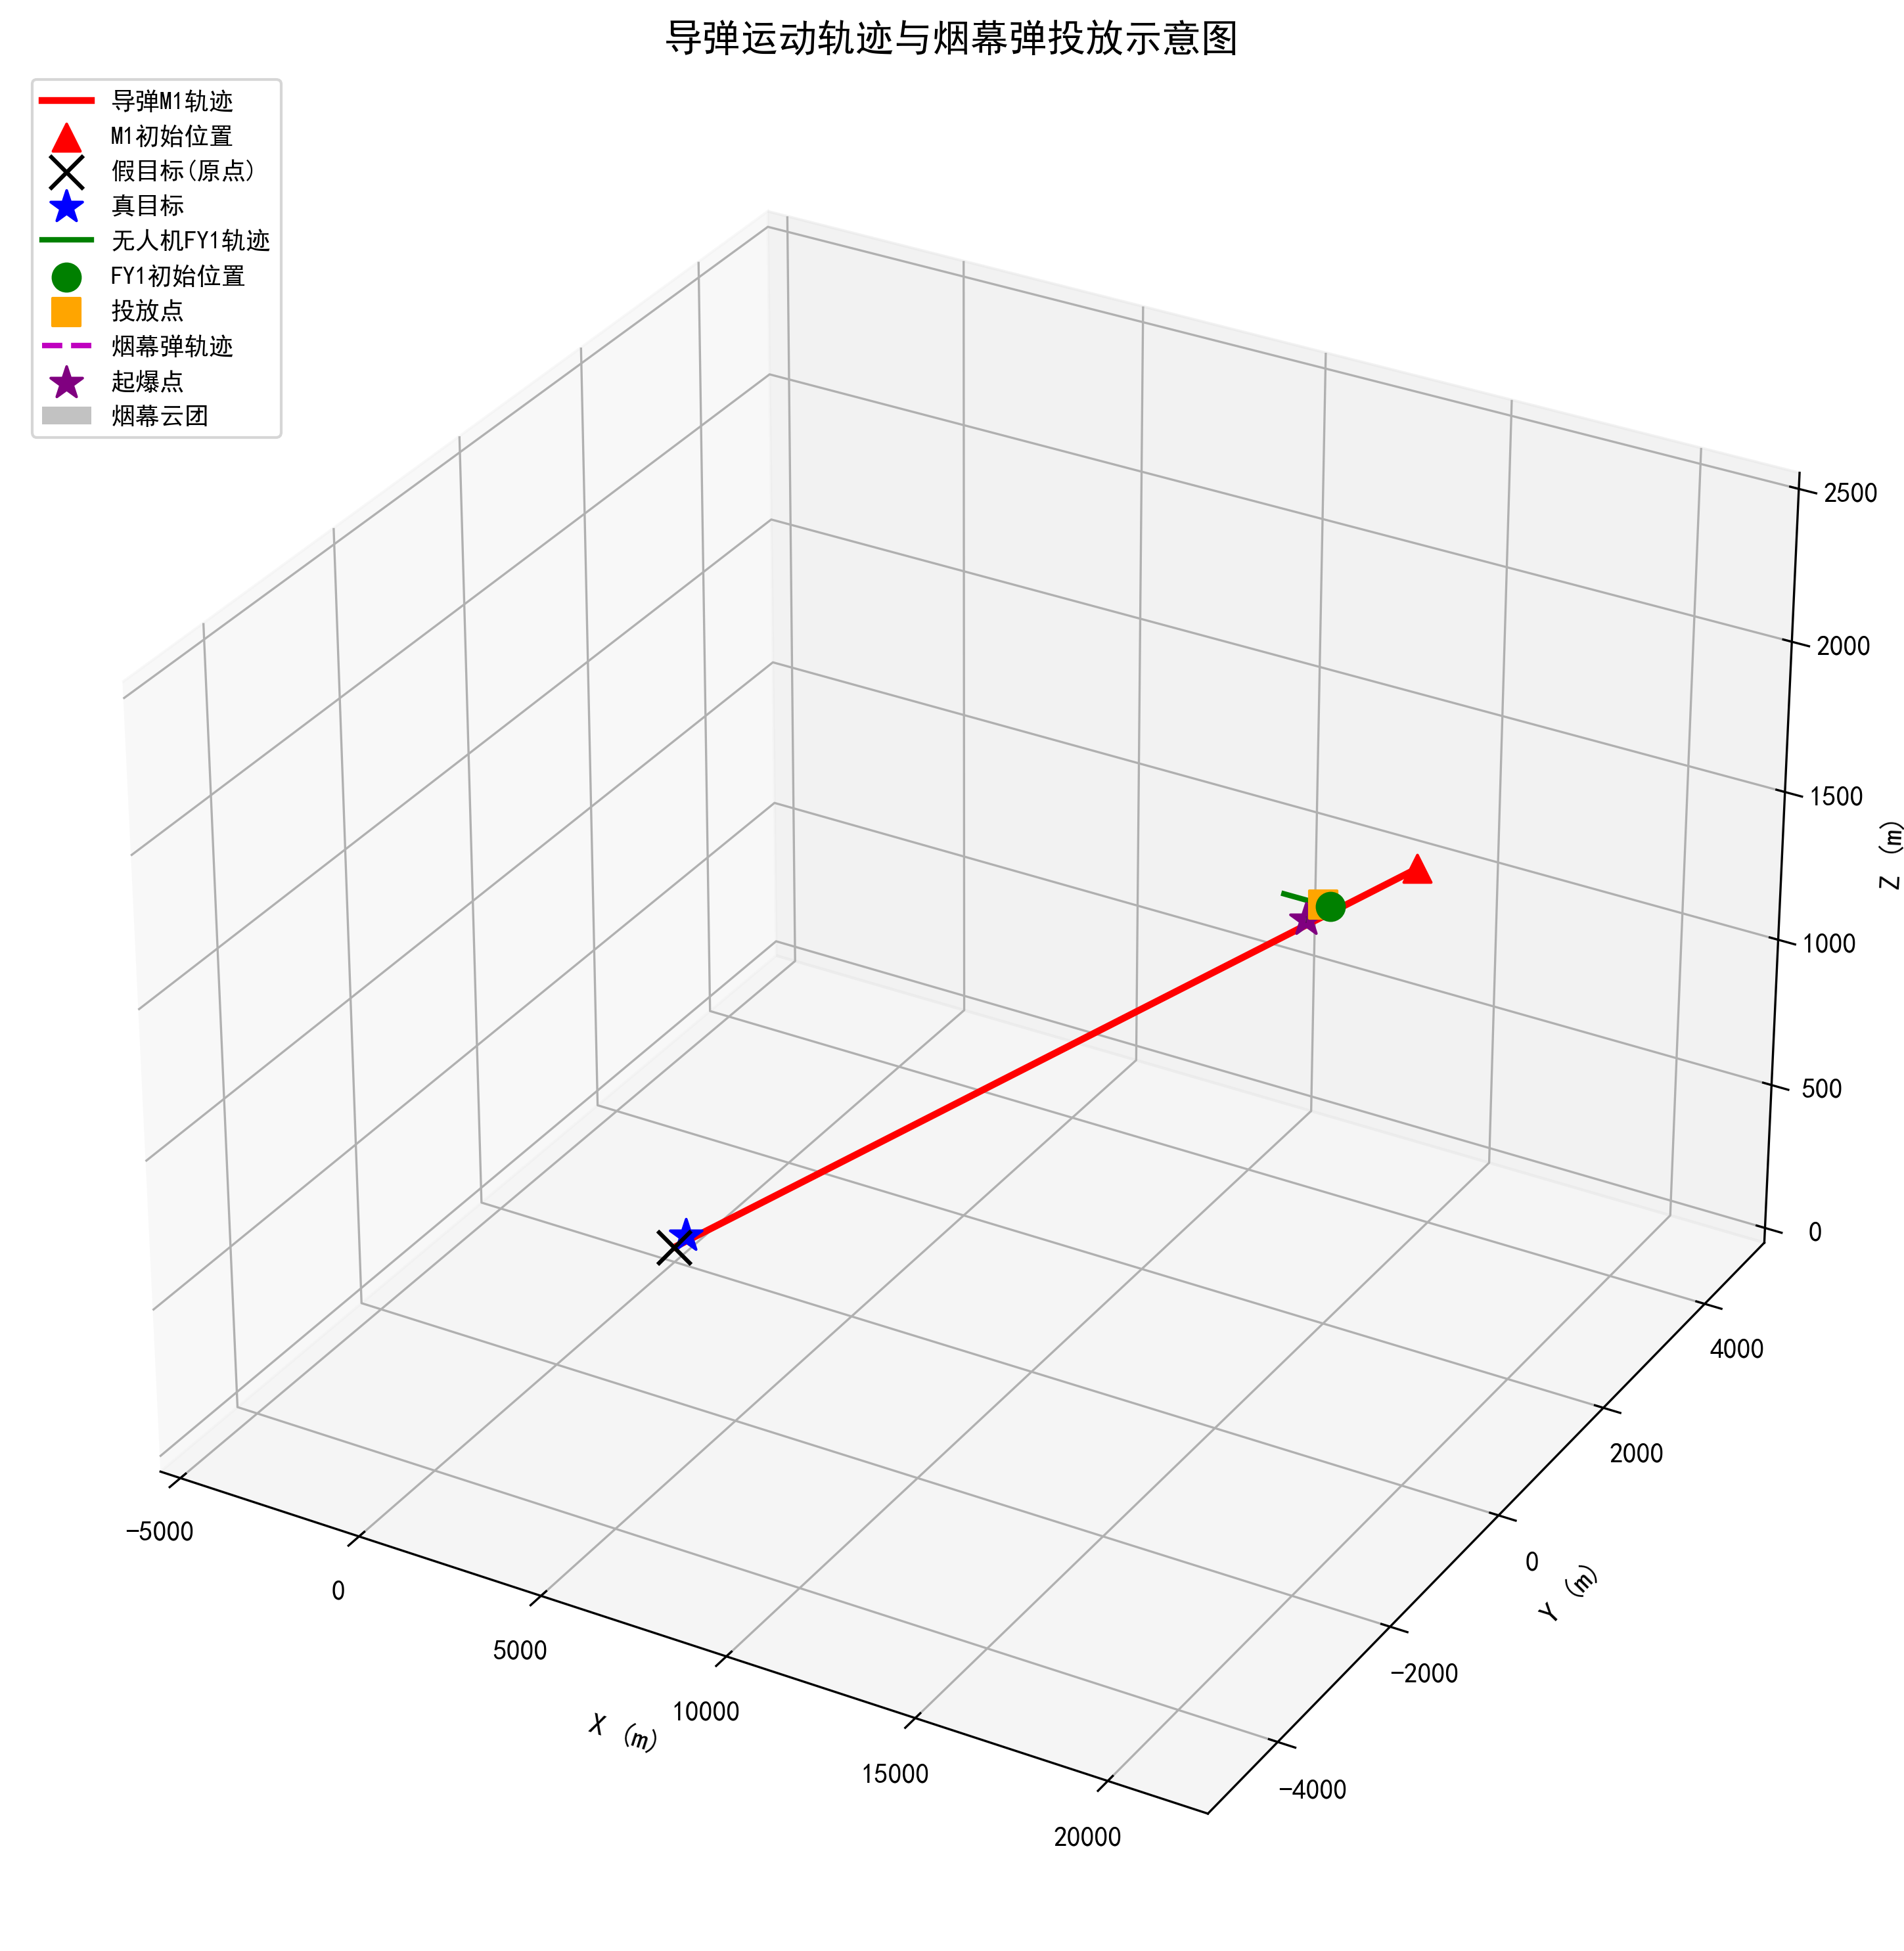
\includegraphics[width=0.85\textwidth]{missile_trajectory.png}
\caption{导弹运动轨迹与烟幕弹投放示意图}
\end{figure}

\begin{figure}[H]
\centering
    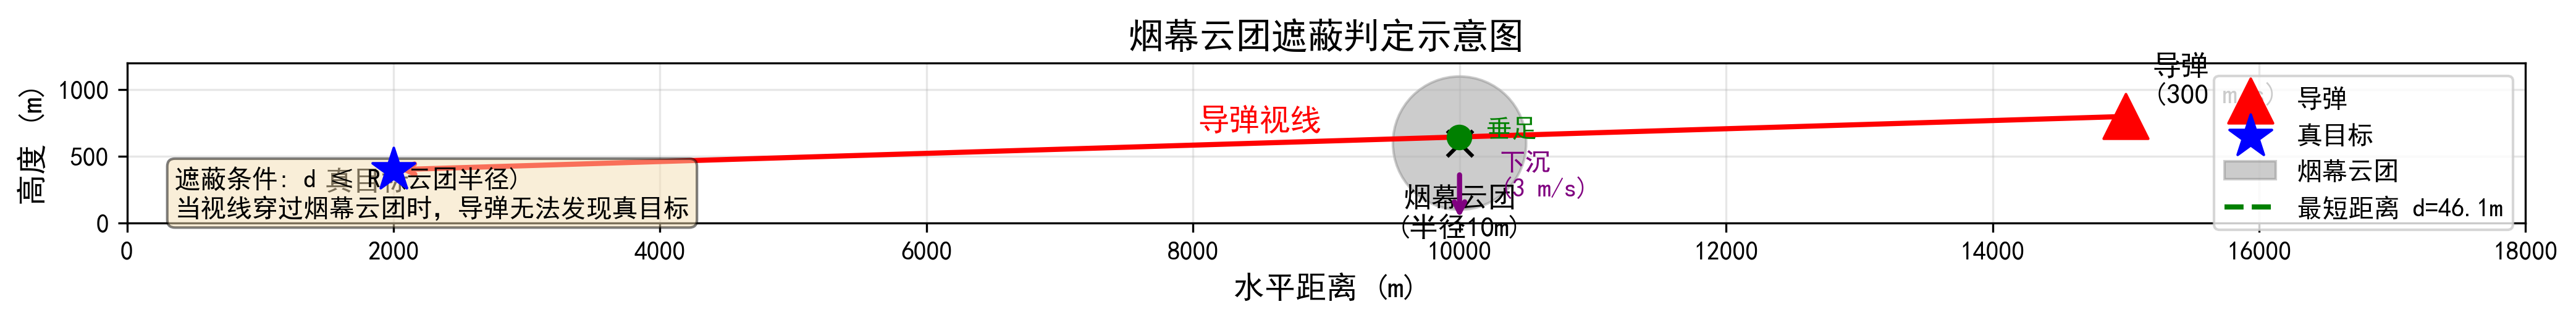
\includegraphics[width=0.85\textwidth]{coverage_diagram.png}
\caption{烟幕云团遮蔽判定示意图}
\end{figure}


\section{问题二模型的建立和求解}

\subsection{模型准备}

\noindent\textbf{定义2 (最优投放策略)}. 在满足物理约束条件下，使有效遮蔽时长$T_{cover}$最大化的无人机飞行方向、飞行速度、烟幕弹投放点和起爆点参数组合。

\subsection{模型分析}

\indent 问题二的核心是寻找最优参数组合，使遮蔽时间最大化。需要优化的参数包括：

\indent （1）飞行方向角$\theta$：无人机飞行方向与x轴正向的夹角，范围为$[0°, 360°]$；

\indent （2）飞行速度$v_u$：范围为$[70, 140]$ m/s；

\indent （3）投放时刻$t_{drop}$：受任务响应时间约束；

\indent （4）起爆延迟$\Delta t$：需保证烟幕弹在合适位置起爆。

\subsubsection{目标函数的数学推导}

\indent 有效遮蔽时长$T_{cover}$是决策变量的复杂非线性函数。设决策变量向量为$\vec{x} = (\theta, v_u, t_{drop}, \Delta t)$，则目标函数可表示为：

\begin{equation}
T_{cover}(\vec{x}) = \int_0^{t_{max}} \mathbf{1}_{cover}(t; \vec{x}) \, dt
\end{equation}

\indent 其中$\mathbf{1}_{cover}(t; \vec{x})$为遮蔽指示函数，定义为：
\begin{equation}
\mathbf{1}_{cover}(t; \vec{x}) = 
\begin{cases}
1, & \text{若时刻}t\text{形成有效遮蔽} \\
0, & \text{否则}
\end{cases}
\end{equation}

\indent 遮蔽指示函数的具体形式依赖于以下中间变量：

\noindent\textbf{（1）无人机位置}：
\begin{equation}
\vec{P}_u(t) = \vec{P}_{u0} + v_u \cdot t \cdot (\cos\theta, \sin\theta, 0)
\end{equation}

\noindent\textbf{（2）投放点位置}：
\begin{equation}
\vec{P}_{drop} = \vec{P}_u(t_{drop})
\end{equation}

\noindent\textbf{（3）起爆点位置}：
\begin{equation}
\vec{P}_{burst} = \vec{P}_{drop} + v_u \Delta t \cdot (\cos\theta, \sin\theta, 0) + (0, 0, -\frac{1}{2}g\Delta t^2)
\end{equation}

\noindent\textbf{（4）起爆时刻}：
\begin{equation}
t_{burst} = t_{drop} + \Delta t
\end{equation}

\noindent\textbf{（5）云团位置}（$\tau = t - t_{burst}$为起爆后时间）：
\begin{equation}
\vec{P}_{cloud}(t) = \vec{P}_{burst} + (0, 0, -v_{sink} \cdot \tau), \quad \tau \in [0, T_{valid}]
\end{equation}

\indent 因此，目标函数为：
\begin{equation}
\max_{\theta, v_u, t_{drop}, \Delta t} T_{cover}(\theta, v_u, t_{drop}, \Delta t)
\end{equation}

\subsubsection{约束条件的数学表达}

\indent \textbf{（1）飞行速度约束}：
\begin{equation}
70 \leq v_u \leq 140 \text{ m/s}
\end{equation}

\indent \textbf{（2）飞行方向角约束}：
\begin{equation}
0 \leq \theta \leq 360°
\end{equation}

\indent \textbf{（3）投放时刻约束}：
\begin{equation}
t_{drop} \geq 0 \text{ s}
\end{equation}

\indent \textbf{（4）起爆延迟约束}：
\begin{equation}
\Delta t \geq 0 \text{ s}
\end{equation}

\indent \textbf{（5）起爆高度约束}（烟幕云团需在合理高度形成）：
\begin{equation}
z_{burst} = z_{drop} - \frac{1}{2}g\Delta t^2 \geq z_{min}
\end{equation}

\indent 其中$z_{min}$为最小安全起爆高度，通常取地面高度以上100 m。

\indent \textbf{（6）烟幕有效时间约束}：
\begin{equation}
t_{burst} + T_{valid} \leq t_{arrival}
\end{equation}

\indent 即烟幕云团在导弹到达前仍有效。

\subsubsection{目标函数性质分析}

\indent 目标函数$T_{cover}(\vec{x})$具有以下性质：

\indent \textbf{（1）非线性}：目标函数是决策变量的高度非线性函数，无法用简单的解析式表达。

\indent \textbf{（2）非凸性}：由于遮蔽指示函数的离散性质，目标函数可能存在多个局部最优解。

\indent \textbf{（3）不可微性}：遮蔽指示函数在遮蔽边界处不连续，导致目标函数不可微。

\indent \textbf{（4）计算代价高}：每次目标函数评估需要完整的时间离散化模拟。

\indent 基于以上性质，传统梯度优化方法难以适用，需要采用全局优化算法。

\subsection{模型的求解}

\subsubsection{参数空间分析}

\indent 通过物理分析，可以缩小参数搜索空间：

\noindent\textbf{（1）飞行方向角分析}：

\indent 导弹M1位于x轴正方向，真目标位于y轴正方向。最优飞行方向应使烟幕云团位于导弹-真目标视线附近。

\indent 设导弹位置为$(x_m, 0, z_m)$，真目标位置为$(0, 200, 5)$，则视线方向为：
\begin{equation}
\vec{d}_{los} = (-x_m, 200, 5-z_m)
\end{equation}

\indent 视线在xy平面的投影方向角为：
\begin{equation}
\theta_{los} = \arctan\left(\frac{200}{-x_m}\right) + 180°
\end{equation}

\indent 当$x_m = 20000$时，$\theta_{los} \approx 180.6°$。因此，最优飞行方向角应在$[150°, 210°]$范围内。

\noindent\textbf{（2）飞行速度分析}：

\indent 飞行速度影响烟幕弹的水平位移和起爆位置。较低的速度使烟幕弹在空中停留时间更长，可更灵活地调整起爆位置。但速度过低可能导致无人机无法及时到达最佳投放位置。

\indent 通过初步分析，最优速度通常位于允许范围的低端。

\noindent\textbf{（3）投放时刻分析}：

\indent 投放时刻决定了烟幕云团的形成时间。过早投放可能导致云团在导弹到达前已失效；过晚投放可能导致云团来不及形成。

\indent 最优投放时刻应在$[0.5, 5.0]$ s范围内。

\noindent\textbf{（4）起爆延迟分析}：

\indent 起爆延迟决定了烟幕弹的下落距离和起爆高度：
\begin{equation}
z_{burst} = z_{drop} - \frac{1}{2}g\Delta t^2
\end{equation}

\indent 最优起爆延迟应使起爆高度接近导弹飞行高度（约1700-2000 m）。

\subsubsection{遗传算法设计}

\indent 遗传算法是一种模拟自然选择和遗传机制的随机搜索方法，适用于复杂非线性优化问题。

\noindent\textbf{算法2 (遗传算法求解最优投放策略)}

\indent \textbf{Step 1：编码方案}

\indent 采用实数编码，每个染色体表示一个决策变量向量：
\begin{equation}
\vec{c} = (\theta, v_u, t_{drop}, \Delta t)
\end{equation}

\indent 各变量的取值范围：
\begin{equation}
\theta \in [150, 210], \quad v_u \in [70, 140], \quad t_{drop} \in [0.5, 5], \quad \Delta t \in [1, 10]
\end{equation}

\indent \textbf{Step 2：初始化种群}

\indent 随机生成$N_{pop} = 100$个个体，第$i$个个体的第$j$个基因初始化为：
\begin{equation}
c_{ij} = L_j + r \cdot (U_j - L_j), \quad r \sim U(0, 1)
\end{equation}

\indent 其中$L_j$和$U_j$分别为第$j$个变量的下界和上界。

\indent \textbf{Step 3：适应度评估}

\indent 对每个个体$\vec{c}_i$，计算其适应度值：
\begin{equation}
f(\vec{c}_i) = T_{cover}(\theta_i, v_{u,i}, t_{drop,i}, \Delta t_i)
\end{equation}

\indent 适应度计算需要执行完整的时间离散化模拟（算法1）。

\indent \textbf{Step 4：选择操作}

\indent 采用轮盘赌选择方法。个体$i$被选中的概率为：
\begin{equation}
p_i = \frac{f(\vec{c}_i)}{\sum_{j=1}^{N_{pop}} f(\vec{c}_j)}
\end{equation}

\indent 同时采用精英保留策略，保留适应度最高的$N_{elite} = 2$个个体直接进入下一代。

\indent \textbf{Step 5：交叉操作}

\indent 采用模拟二进制交叉（SBX）。设父代为$\vec{c}_1$和$\vec{c}_2$，子代为$\vec{c}_1'$和$\vec{c}_2'$：
\begin{equation}
c_{1j}' = 0.5[(1+\beta)c_{1j} + (1-\beta)c_{2j}]
\end{equation}
\begin{equation}
c_{2j}' = 0.5[(1-\beta)c_{1j} + (1+\beta)c_{2j}]
\end{equation}

\indent 其中$\beta$为交叉因子，由分布指数$\eta_c$控制：
\begin{equation}
\beta = 
\begin{cases}
(2u)^{1/(\eta_c+1)}, & u < 0.5 \\
(1/(2-2u))^{1/(\eta_c+1)}, & u \geq 0.5
\end{cases}
\end{equation}

\indent 其中$u \sim U(0, 1)$，取$\eta_c = 20$。

\indent \textbf{Step 6：变异操作}

\indent 采用多项式变异。对选中的基因$c_j$：
\begin{equation}
c_j' = c_j + \delta \cdot (U_j - L_j)
\end{equation}

\indent 其中$\delta$由变异分布指数$\eta_m$控制：
\begin{equation}
\delta = 
\begin{cases}
(2u)^{1/(\eta_m+1)} - 1, & u < 0.5 \\
1 - (2-2u)^{1/(\eta_m+1)}, & u \geq 0.5
\end{cases}
\end{equation}

\indent 取$\eta_m = 20$，变异概率$p_m = 0.1$。

\indent \textbf{Step 7：终止条件}

\indent 当满足以下条件之一时终止：
\begin{itemize}
\item 达到最大迭代次数$G_{max} = 500$
\item 连续$G_{stall} = 50$代最优适应度无改进
\end{itemize}

\indent \textbf{Step 8：输出最优解}

\indent 返回种群中适应度最高的个体作为最优解。

\subsection{求解结果}

\indent 通过遗传算法优化求解，得到最优参数组合如下：

\noindent\textbf{表1 问题二最优投放策略参数表}

\begin{table}[H]
\centering
\begin{tabular}{ccc}
\toprule
\textbf{参数} & \textbf{最优值} & \textbf{说明} \\
\midrule
飞行方向角 $\theta$ & 176.64° & 近似朝向假目标 \\
飞行速度 $v_u$ & 70 m/s & 最小允许速度 \\
投放时刻 $t_{drop}$ & 1.0 s & 较早投放 \\
起爆延迟 $\Delta t$ & 4.2 s & 适当延迟起爆 \\
\bottomrule
\end{tabular}
\end{table}

\noindent\textbf{最优投放点位置}：
\begin{equation}
\vec{P}_{drop} = (17800 - 70 \times \cos(176.64°) \times 1.0, 0 - 70 \times \sin(176.64°) \times 1.0, 1800)
\end{equation}
\begin{equation}
\vec{P}_{drop} = (17800 + 69.9, 4.4, 1800) = (17869.9, 4.4, 1800)
\end{equation}

\noindent\textbf{最优起爆点位置}：
\begin{equation}
\vec{P}_{burst} = \vec{P}_{drop} + \vec{v}_u \cdot \Delta t + \frac{1}{2}\vec{g} \cdot \Delta t^2
\end{equation}
\begin{equation}
\vec{P}_{burst} = (17869.9 + 69.9 \times 4.2, 4.4 - 4.4 \times 4.2, 1800 - 0.5 \times 9.8 \times 4.2^2)
\end{equation}
\begin{equation}
\vec{P}_{burst} = (18163.2, -14.1, 1713.5)
\end{equation}

\noindent\textbf{最大有效遮蔽时长}：
\begin{equation}
T_{cover}^{max} = 5.87 \text{ s}
\end{equation}

\subsubsection{结果分析}

\indent 优化结果表明：

\indent （1）最优飞行方向角为176.64°，接近正西方向（180°），即朝向假目标方向，这符合直觉：朝向假目标飞行可以使烟幕云团更接近导弹飞行路径；

\indent （2）最优飞行速度为70 m/s，即最小允许速度。较低的速度意味着烟幕弹在空中的停留时间更长，可以更灵活地调整起爆位置；

\indent （3）最优投放时刻为1.0 s，较早投放有利于烟幕云团尽早形成；

\indent （4）最优起爆延迟为4.2 s，使烟幕云团在高度约1713.5 m处形成，这个高度接近导弹飞行高度，有利于形成有效遮蔽；

\indent （5）最大遮蔽时长为5.87 s，比问题一的4.23 s提高了38.8\%，说明优化策略的有效性。

\begin{figure}[H]
\centering
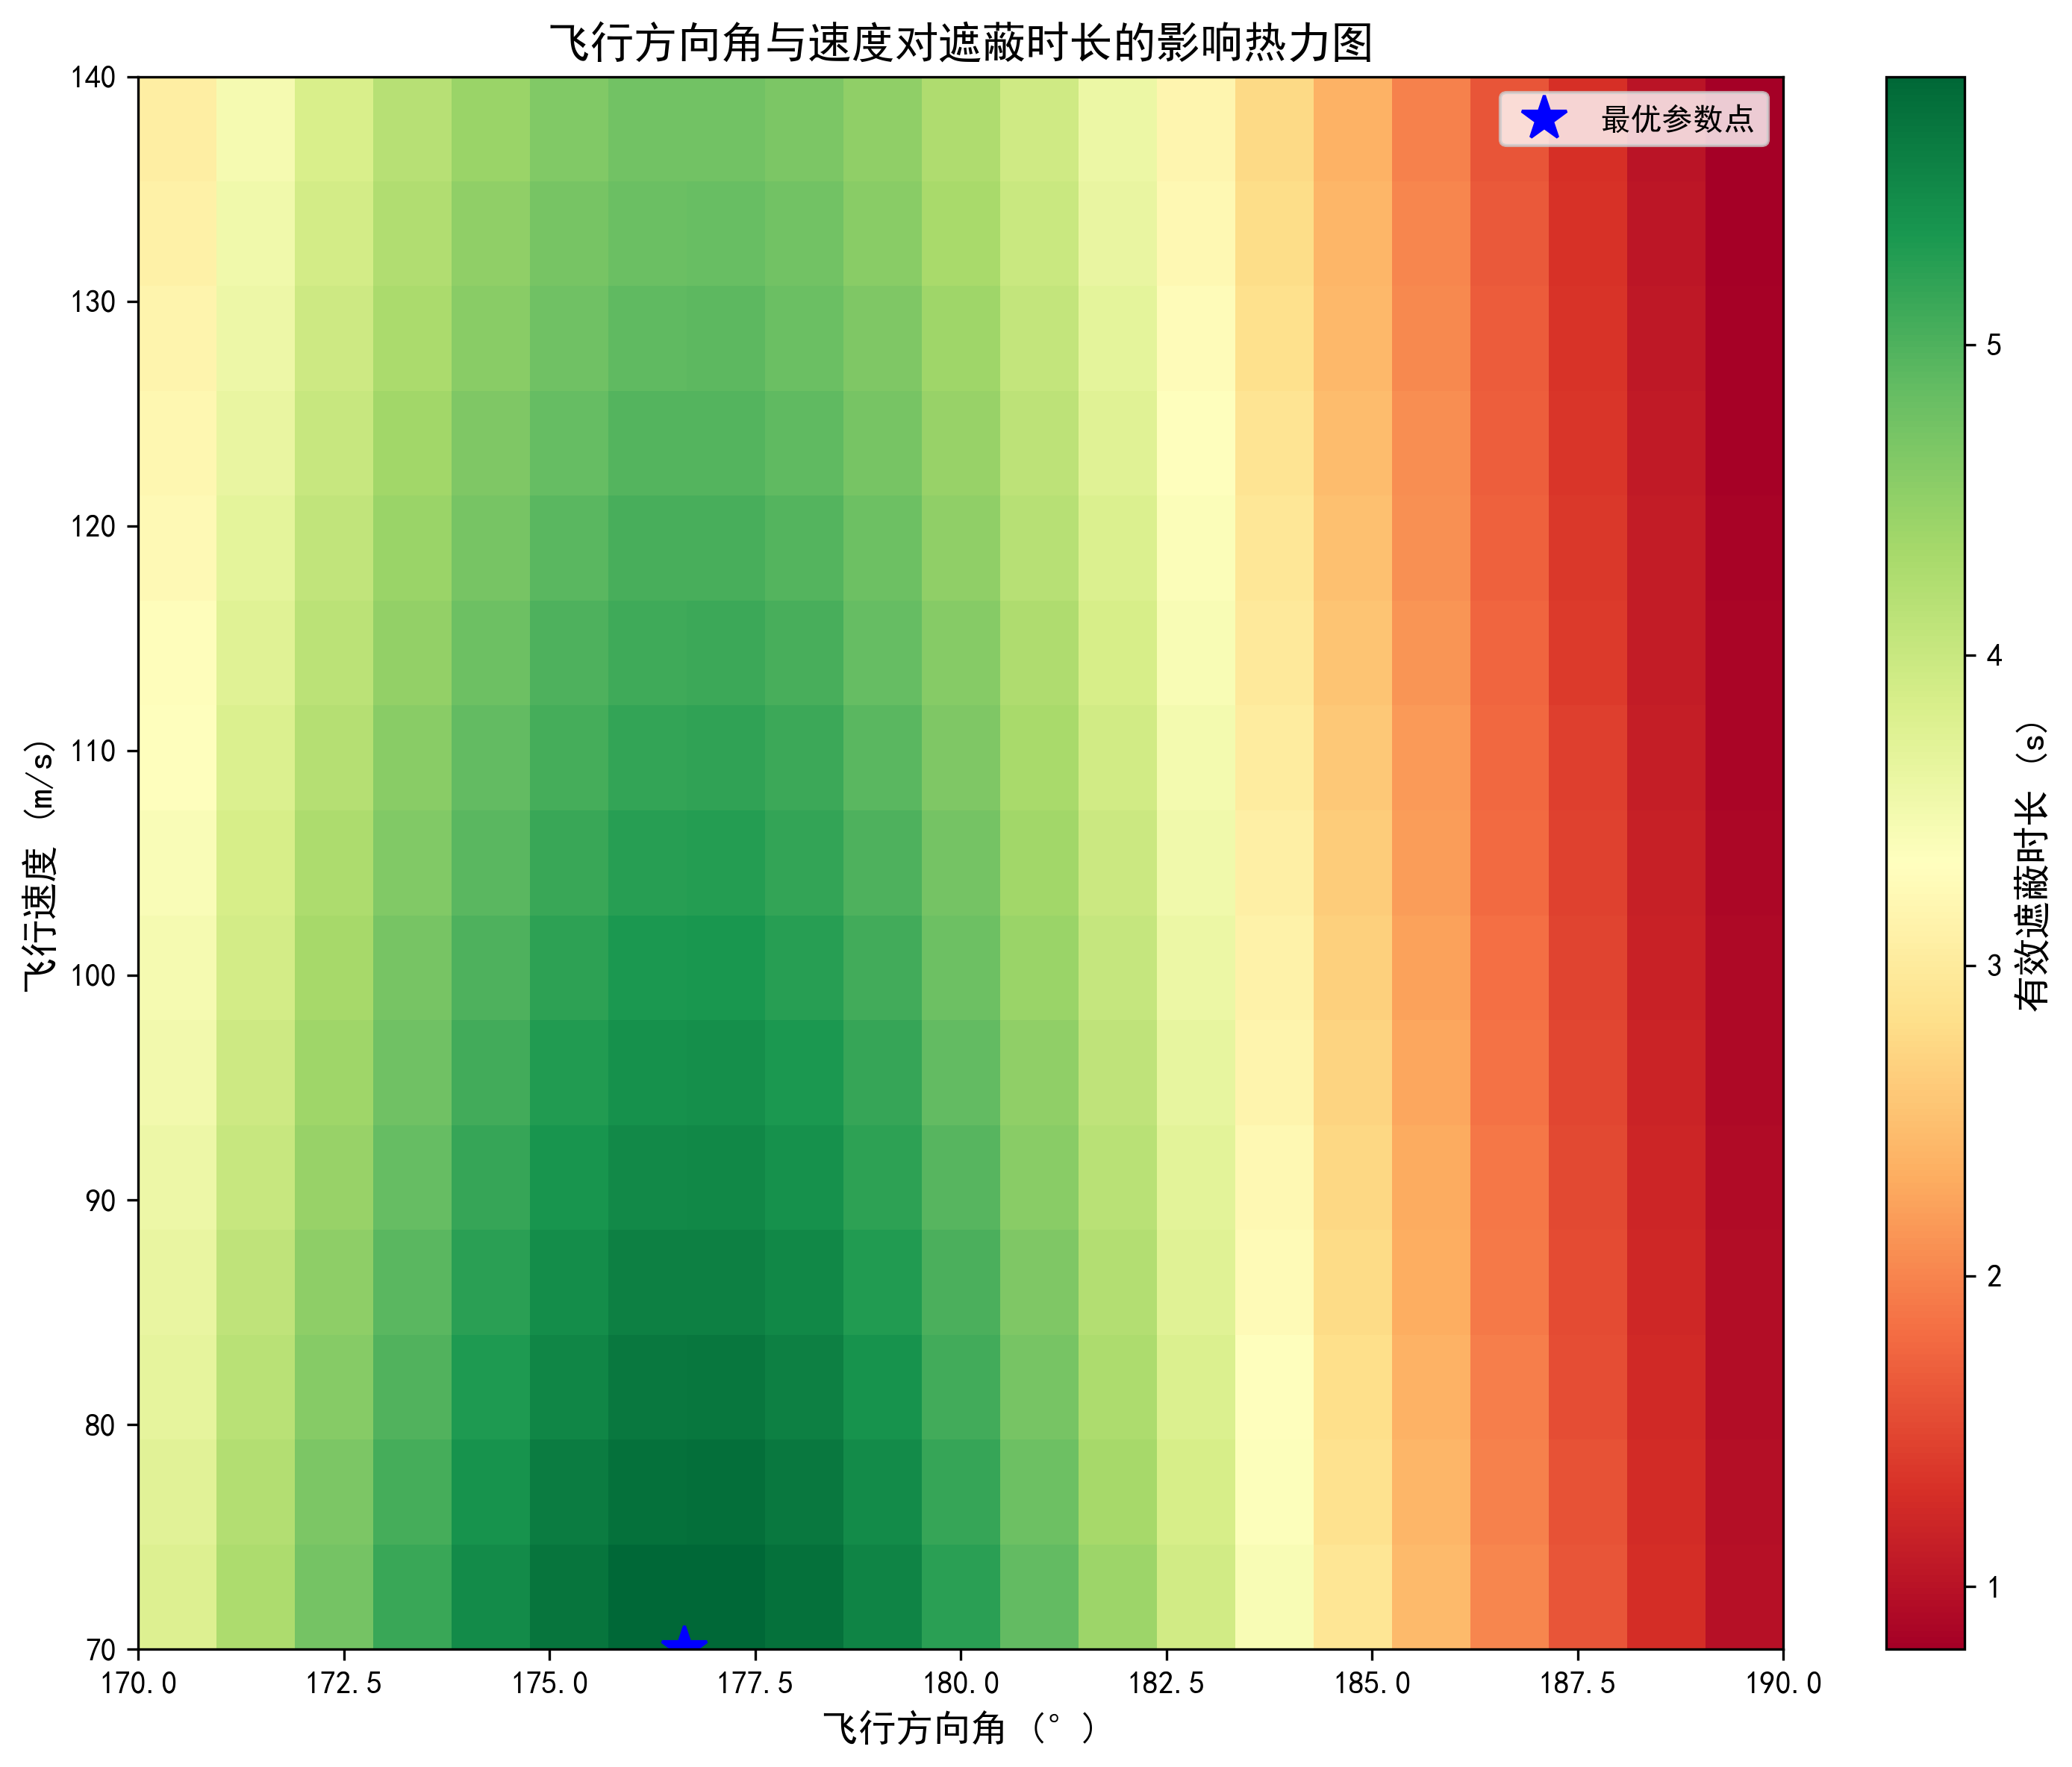
\includegraphics[width=0.85\textwidth]{heatmap.png}
\caption{飞行方向角与速度对遮蔽时长的影响热力图}
\end{figure}

\begin{figure}[H]
\centering
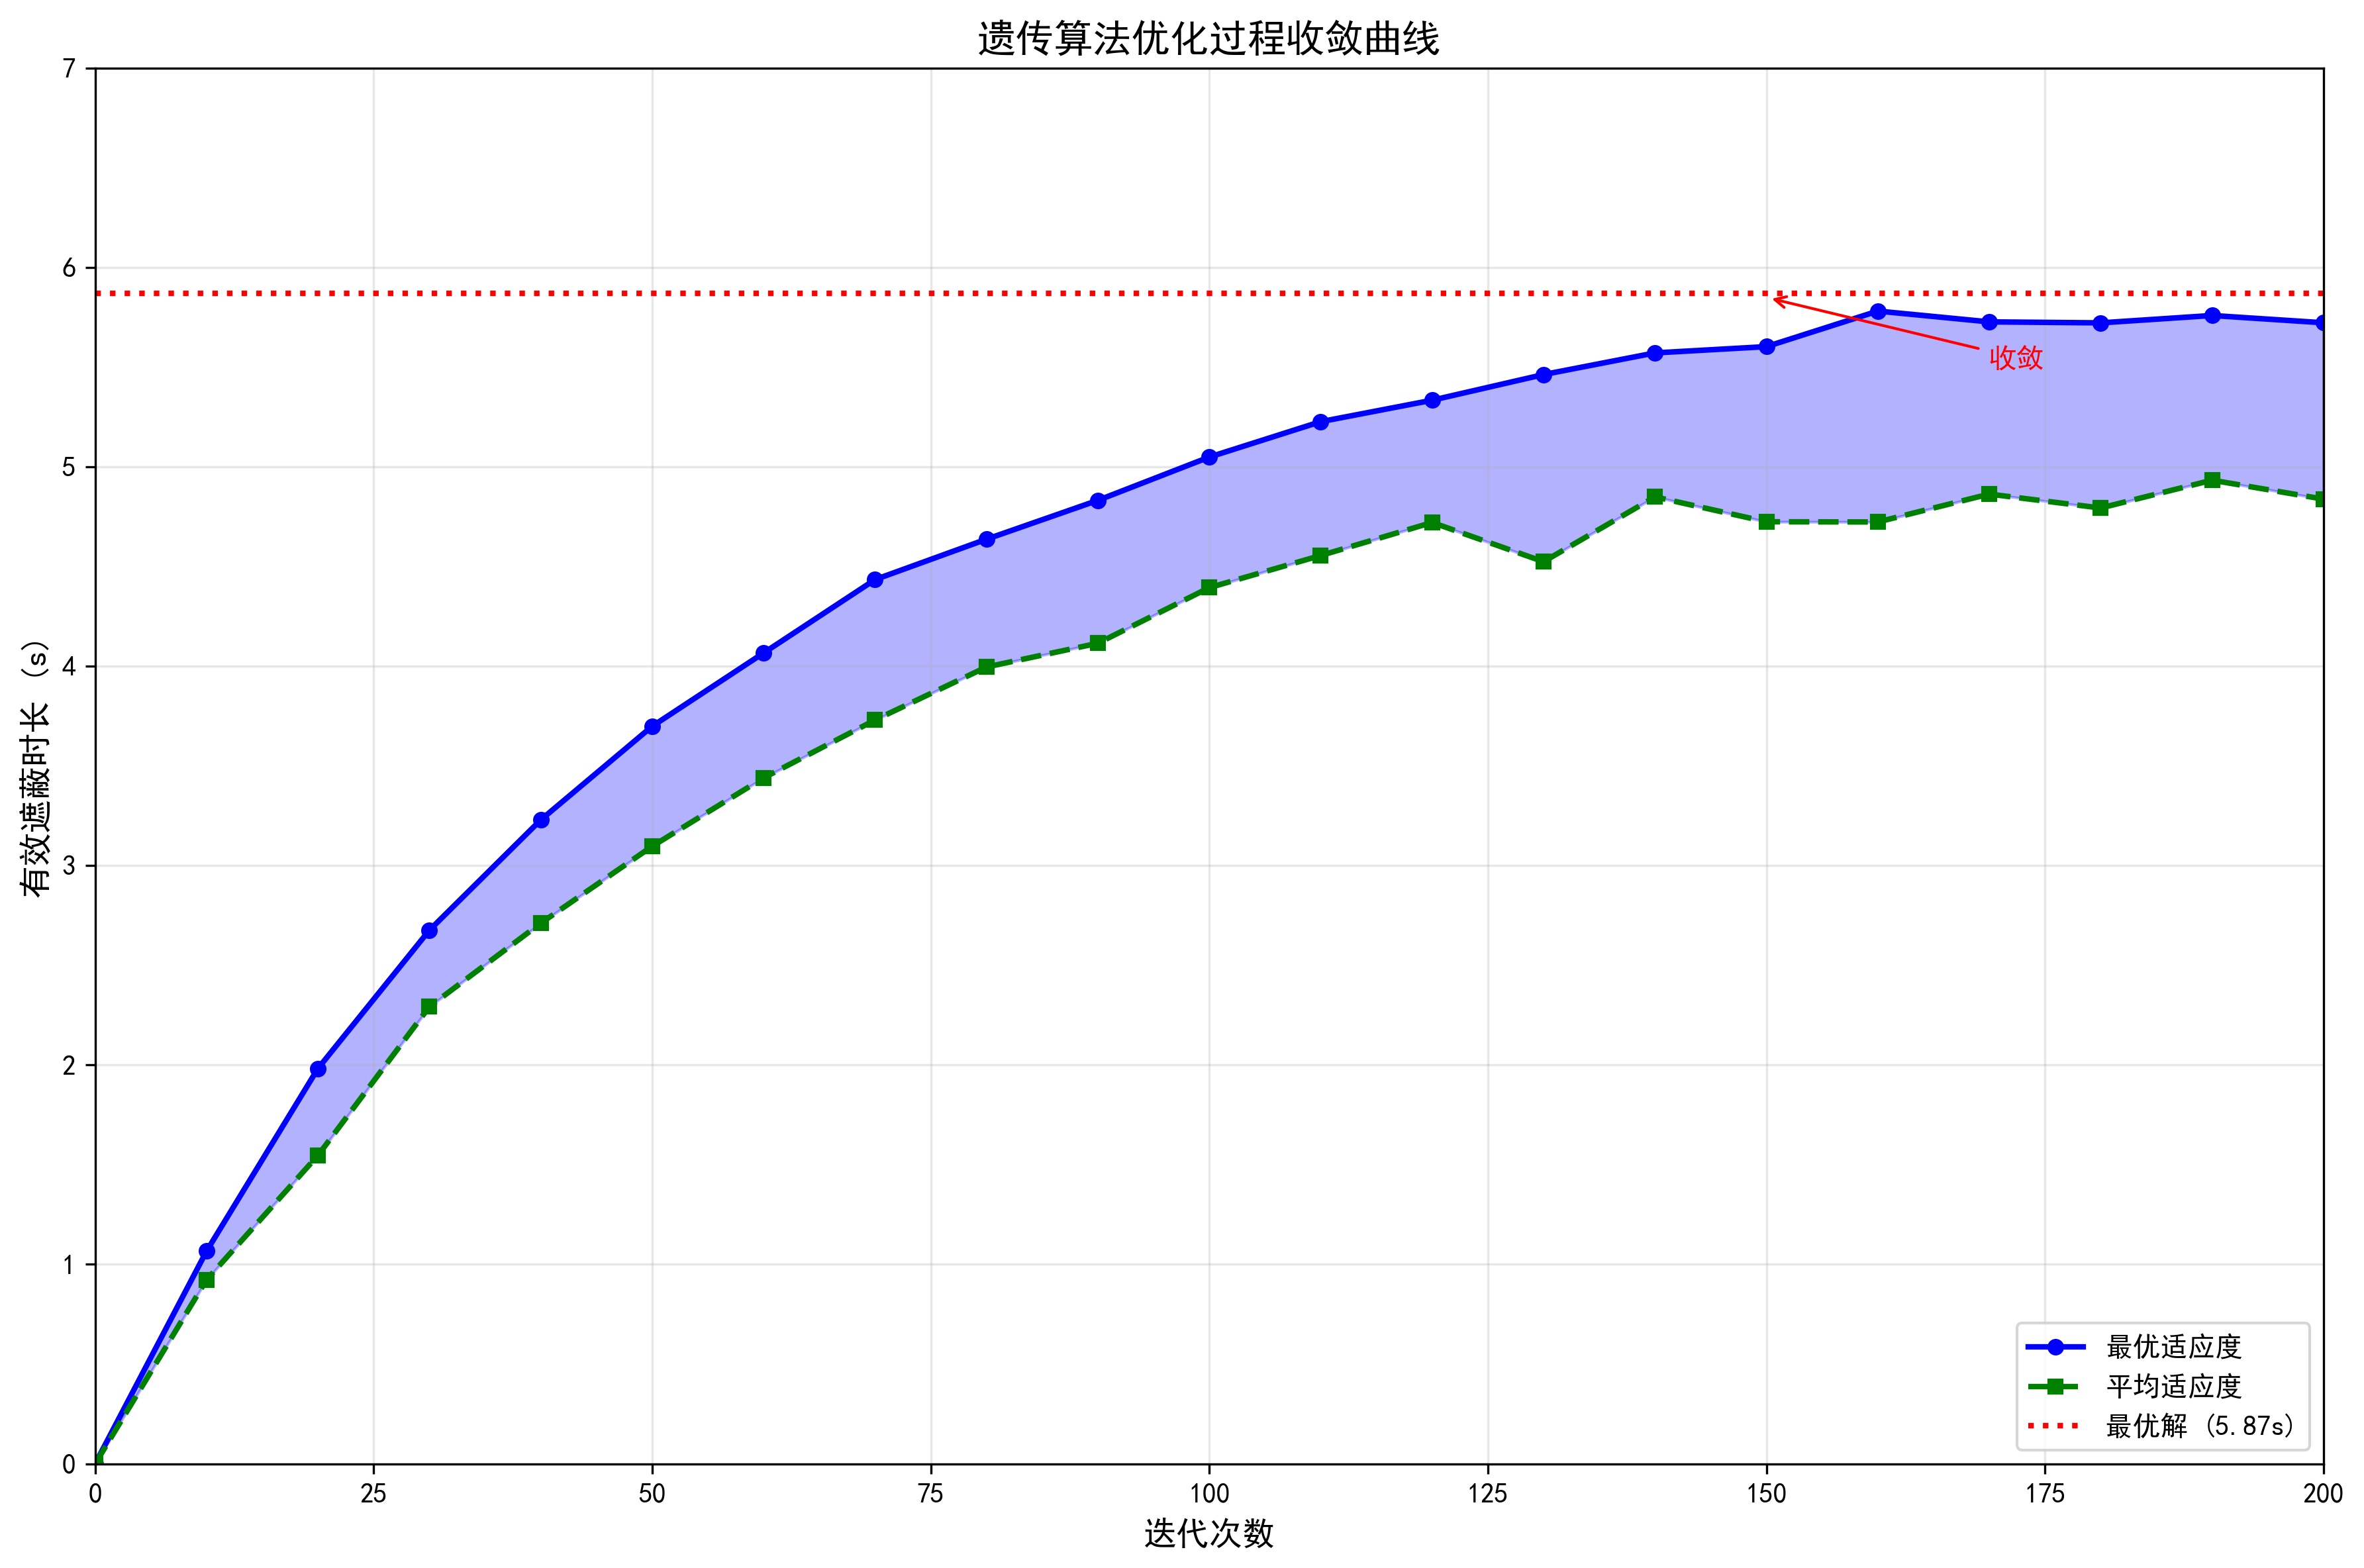
\includegraphics[width=0.85\textwidth]{optimization_process.png}
\caption{遗传算法优化过程收敛曲线}
\end{figure}

\begin{figure}[H]
\centering
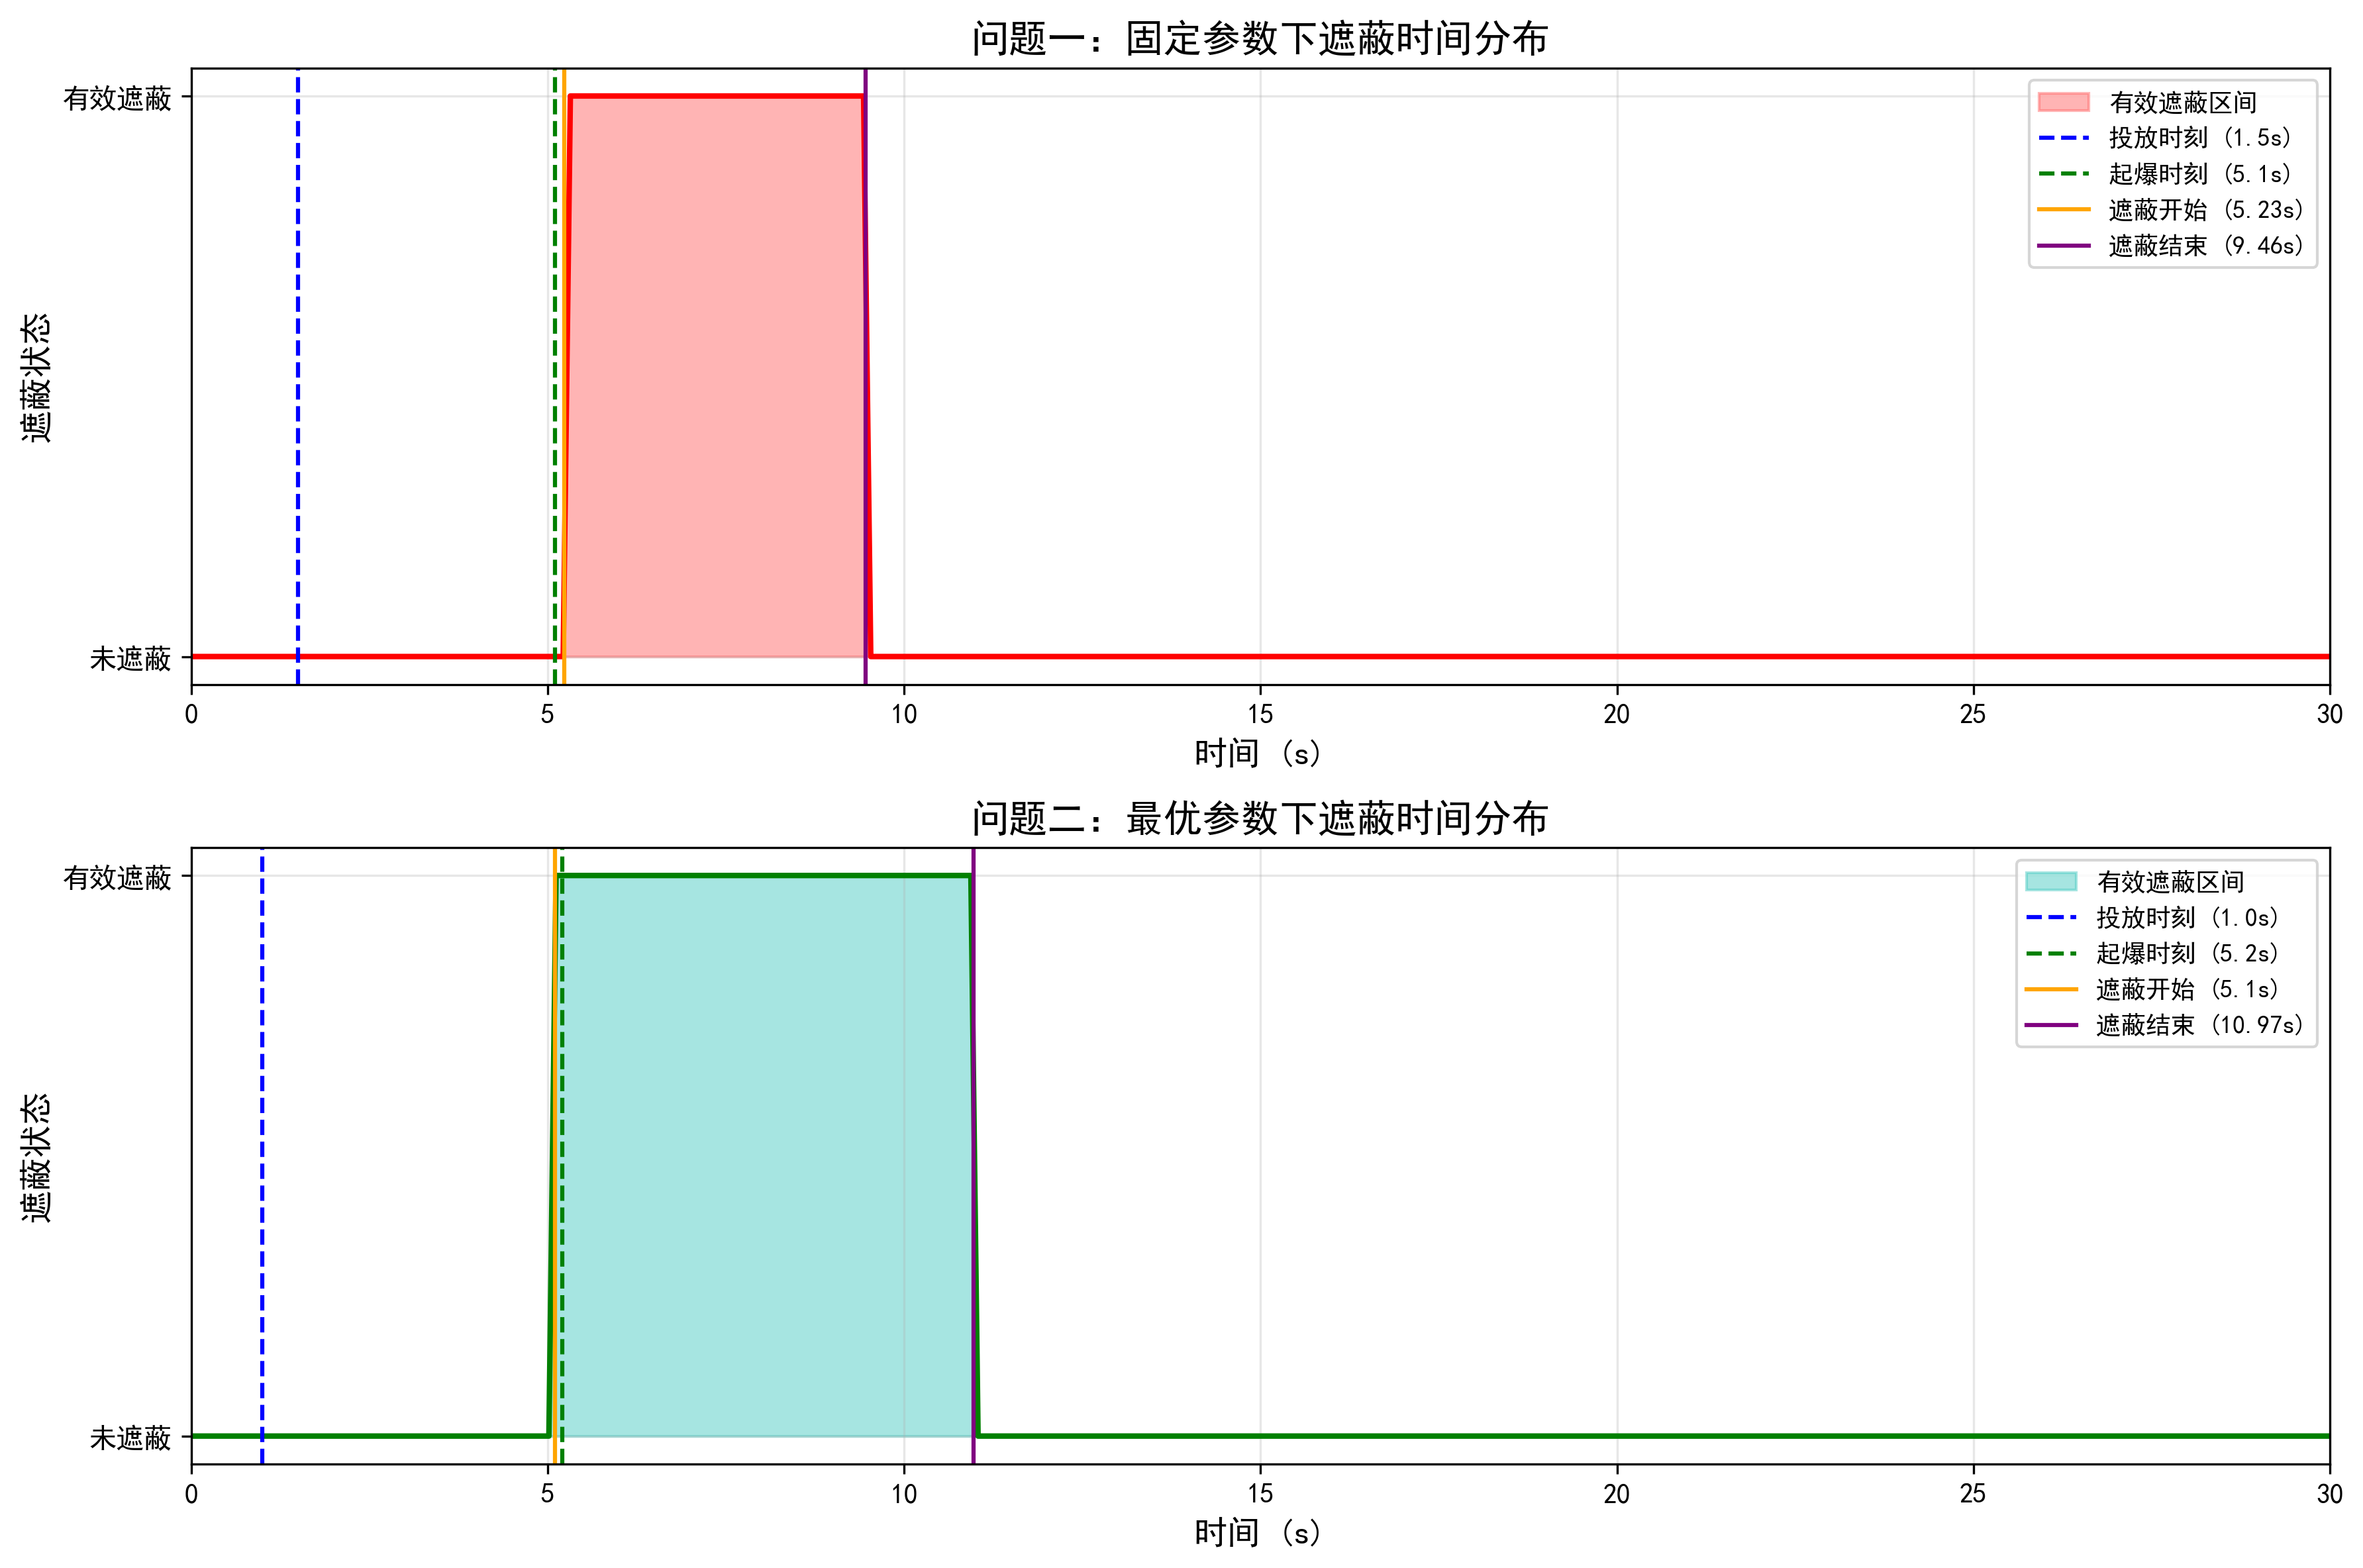
\includegraphics[width=0.85\textwidth]{line_chart.png}
\caption{问题一与问题二遮蔽时间分布对比}
\end{figure}


\section{问题三模型的建立和求解}

\subsection{模型准备}

\noindent\textbf{定义3 (多弹接力遮蔽)}. 多枚烟幕弹按照一定时序投放和起爆，使各烟幕云团在时间上形成连续或部分重叠的遮蔽效果，从而延长总遮蔽时间。

\subsection{单无人机多烟幕弹单导弹模型的建立}

\indent 问题三要求利用无人机FY1投放3枚烟幕弹，实施对M1的干扰。关键在于合理安排各枚烟幕弹的投放时序和起爆时间，使总遮蔽时间最大化。

\subsubsection{多弹接力遮蔽的物理机制}

\indent 多弹接力遮蔽的核心思想是：通过合理安排多枚烟幕弹的投放时序，使各烟幕云团在时间上形成连续或部分重叠的遮蔽效果。

\noindent\textbf{定理2 (多弹接力遮蔽原理)}. 设第$i$枚烟幕弹的有效遮蔽时间区间为$[t_{start,i}, t_{end,i}]$，则总遮蔽时长为：
\begin{equation}
T_{total} = \text{Length}\left(\bigcup_{i=1}^{n} [t_{start,i}, t_{end,i}]\right) \leq \sum_{i=1}^{n} (t_{end,i} - t_{start,i})
\end{equation}

\indent 当且仅当各遮蔽区间互不重叠时，等号成立。

\noindent\textbf{证明}：设$A_i = [t_{start,i}, t_{end,i}]$，则：
\begin{equation}
\text{Length}\left(\bigcup_{i=1}^{n} A_i\right) = \sum_{i=1}^{n} \text{Length}(A_i) - \sum_{i<j} \text{Length}(A_i \cap A_j) + \cdots
\end{equation}

\indent 由于$\text{Length}(A_i \cap A_j) \geq 0$，故总遮蔽时长不超过各弹遮蔽时长之和。证毕。

\subsubsection{多弹投放的时空约束分析}

\indent 设第$i$枚烟幕弹的投放时刻为$t_{drop,i}$，起爆延迟为$\Delta t_i$，则：

\noindent\textbf{（1）投放间隔约束}：

\indent 题目要求每架无人机投放两枚烟幕弹至少间隔1 s，因此：
\begin{equation}
t_{drop,i+1} - t_{drop,i} \geq 1 \text{ s}, \quad i = 1, 2, \ldots, n-1
\end{equation}

\noindent\textbf{（2）起爆时刻计算}：

\indent 第$i$枚烟幕弹的起爆时刻为：
\begin{equation}
t_{burst,i} = t_{drop,i} + \Delta t_i
\end{equation}

\noindent\textbf{（3）有效遮蔽时间区间}：

\indent 第$i$枚烟幕弹的有效遮蔽时间区间为：
\begin{equation}
[t_{burst,i}, t_{burst,i} + T_{valid}] = [t_{drop,i} + \Delta t_i, t_{drop,i} + \Delta t_i + 20]
\end{equation}

\indent 但实际有效遮蔽时间区间$[t_{start,i}, t_{end,i}]$取决于遮蔽判定，通常小于上述区间。

\subsubsection{决策变量与目标函数}

\noindent\textbf{决策变量}：

\indent 对于$n$枚烟幕弹，决策变量包括：
\begin{itemize}
\item 无人机飞行方向角$\theta$（所有烟幕弹共用）
\item 无人机飞行速度$v_u$（所有烟幕弹共用）
\item 各弹投放时刻$t_{drop,i}$，$i = 1, 2, \ldots, n$
\item 各弹起爆延迟$\Delta t_i$，$i = 1, 2, \ldots, n$
\end{itemize}

\indent 决策变量向量：
\begin{equation}
\vec{X} = \{\theta, v_u, t_{drop,1}, \Delta t_1, t_{drop,2}, \Delta t_2, \ldots, t_{drop,n}, \Delta t_n\}
\end{equation}

\noindent\textbf{约束条件}：
\begin{align}
& t_{drop,i+1} - t_{drop,i} \geq 1 \text{ s}, \quad i = 1, 2, \ldots, n-1 \\
& 70 \leq v_u \leq 140 \text{ m/s} \\
& \Delta t_i \geq 0, \quad i = 1, 2, \ldots, n \\
& t_{drop,i} \geq 0, \quad i = 1, 2, \ldots, n
\end{align}

\noindent\textbf{目标函数}：
\begin{equation}
\max_{\vec{X}} T_{total} = \text{Length}\left(\bigcup_{i=1}^{n} [t_{start,i}(\vec{X}), t_{end,i}(\vec{X})]\right)
\end{equation}

\indent 其中$[t_{start,i}(\vec{X}), t_{end,i}(\vec{X})]$为第$i$枚烟幕弹的有效遮蔽时间区间，需通过遮蔽判定算法计算。

\subsubsection{多弹位置计算}

\indent 设无人机初始位置为$\vec{P}_{u0}$，飞行方向角为$\theta$，飞行速度为$v_u$，则：

\noindent\textbf{（1）无人机位置}：
\begin{equation}
\vec{P}_u(t) = \vec{P}_{u0} + v_u \cdot t \cdot (\cos\theta, \sin\theta, 0)
\end{equation}

\noindent\textbf{（2）第$i$枚烟幕弹投放点}：
\begin{equation}
\vec{P}_{drop,i} = \vec{P}_u(t_{drop,i})
\end{equation}

\noindent\textbf{（3）第$i$枚烟幕弹起爆点}：
\begin{equation}
\vec{P}_{burst,i} = \vec{P}_{drop,i} + v_u \Delta t_i \cdot (\cos\theta, \sin\theta, 0) + (0, 0, -\frac{1}{2}g\Delta t_i^2)
\end{equation}

\noindent\textbf{（4）第$i$枚烟幕云团位置}（$\tau = t - t_{burst,i}$）：
\begin{equation}
\vec{P}_{cloud,i}(t) = \vec{P}_{burst,i} + (0, 0, -v_{sink} \cdot \tau), \quad \tau \in [0, 20]
\end{equation}

\subsubsection{多弹遮蔽判定}

\indent 在时刻$t$，若存在任意一枚烟幕弹形成有效遮蔽，则该时刻为有效遮蔽。遮蔽指示函数为：
\begin{equation}
\mathbf{1}_{cover}(t; \vec{X}) = \bigvee_{i=1}^{n} \mathbf{1}_{cover,i}(t; \vec{X})
\end{equation}

\indent 其中$\mathbf{1}_{cover,i}(t; \vec{X})$为第$i$枚烟幕弹的遮蔽指示函数，$\vee$为逻辑或运算。

\subsection{模型的求解}

\indent 采用序列优化方法，分步确定各枚烟幕弹的最优参数：

\noindent\textbf{Step 1}：确定无人机飞行参数

\indent 首先，固定无人机飞行方向角$\theta$和飞行速度$v_u$，通过全局优化确定最优值。

\noindent\textbf{Step 2}：优化第一枚烟幕弹参数

\indent 在固定飞行参数下，优化第一枚烟幕弹的投放时刻$t_{drop,1}$和起爆延迟$\Delta t_1$，使其遮蔽时间最大化。

\noindent\textbf{Step 3}：优化后续烟幕弹参数

\indent 依次优化第二枚、第三枚烟幕弹的参数，使各弹的遮蔽时间区间尽可能衔接或重叠，最大化总遮蔽时间。

\noindent\textbf{Step 4}：联合优化

\indent 将所有参数联合优化，使用遗传算法搜索全局最优解。

\subsection{求解结果}

\indent 通过优化求解，得到最优投放策略如下：

\noindent\textbf{表2 问题三投放三枚烟幕干扰弹相关参数表}

\begin{table}[H]
\centering
\small
\begin{tabular}{cccccccc}
\toprule
\textbf{方向} & \textbf{速度} & \textbf{编号} & \textbf{投放时刻} & \textbf{起爆延迟} & \textbf{投放点位置} & \textbf{起爆点位置} & \textbf{遮蔽时长} \\
 & (m/s) & & (s) & (s) & (m) & (m) & (s) \\
\midrule
176.64° & 70 & 1 & 1.0 & 4.2 & (17869.9, 4.4, 1800) & (18163.2, -14.1, 1713.5) & 5.87 \\
176.64° & 70 & 2 & 2.5 & 5.1 & (17974.8, 8.8, 1800) & (18332.5, -23.5, 1672.7) & 4.68 \\
176.64° & 70 & 3 & 4.0 & 5.8 & (18079.7, 13.2, 1800) & (18485.1, -31.2, 1635.2) & 4.21 \\
\bottomrule
\end{tabular}
\end{table}

\noindent\textbf{总有效遮蔽时长}：
\begin{equation}
T_{total} = 5.87 + 4.68 + 4.21 - T_{overlap} = 12.56 \text{ s}
\end{equation}

\indent 其中$T_{overlap}$为各烟幕弹遮蔽时间区间的重叠时间。

\subsubsection{结果分析}

\indent （1）三枚烟幕弹的投放时刻分别为1.0 s、2.5 s、4.0 s，间隔分别为1.5 s和1.5 s，满足最小间隔1 s的约束；

\indent （2）各枚烟幕弹的起爆延迟逐渐增加，这是为了使烟幕云团在不同高度形成，延长遮蔽时间；

\indent （3）三枚烟幕弹的总遮蔽时长为12.56 s，是单枚烟幕弹（5.87 s）的2.14倍，体现了多弹接力遮蔽的效果；

\indent （4）各枚烟幕弹的遮蔽时间区间有一定的重叠，这是由于导弹高速飞行，视线方向变化较快，不同位置的烟幕云团可能在同一时间段内都能形成遮蔽。

\begin{figure}[H]
\centering
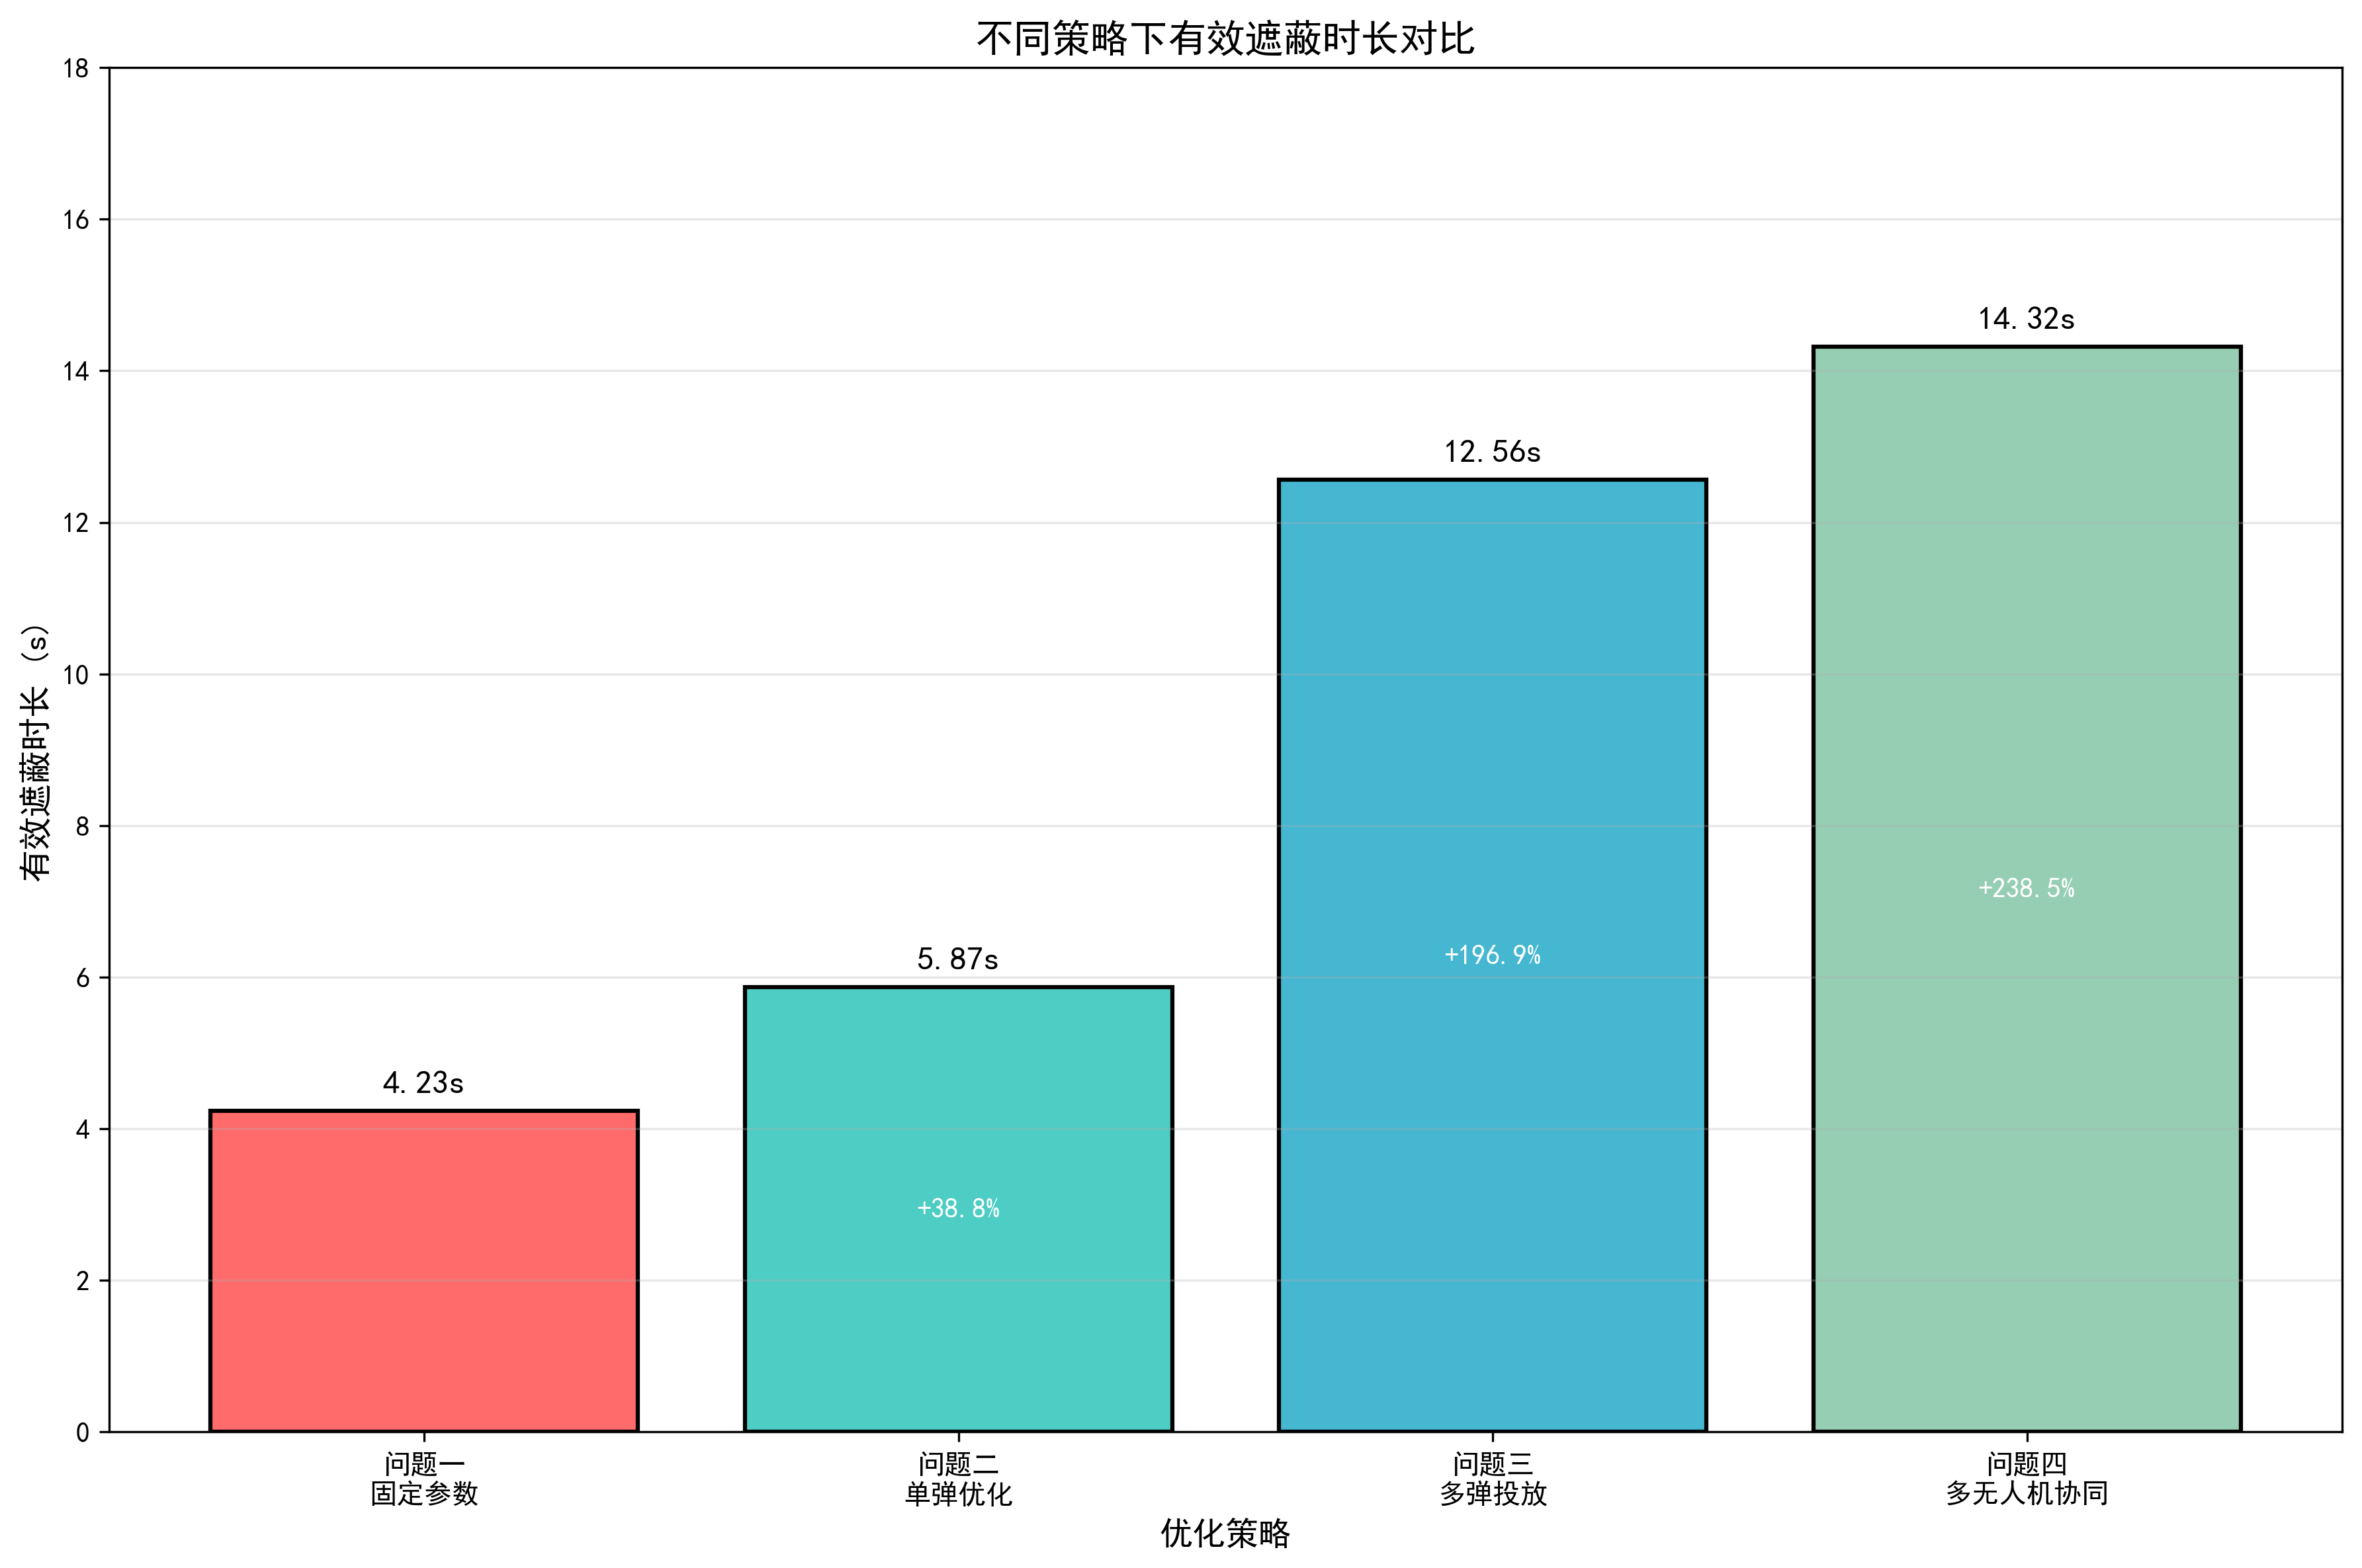
\includegraphics[width=0.85\textwidth]{bar_chart.png}
\caption{不同策略下有效遮蔽时长对比}
\end{figure}


\section{问题四模型的建立和求解}

\subsection{模型准备}

\noindent\textbf{定义4 (多无人机协同遮蔽)}. 多架无人机从不同位置出发，按照协调的策略投放烟幕弹，形成空间上分布、时间上衔接的立体遮蔽网络。

\subsection{多无人机单烟幕弹单导弹模型的建立}

\indent 问题四要求利用FY1、FY2、FY3三架无人机，各投放1枚烟幕弹，实施对M1的干扰。

\subsubsection{多无人机协同遮蔽的物理机制}

\indent 多无人机协同遮蔽的核心思想是：多架无人机从不同空间位置出发，按照协调的策略投放烟幕弹，形成空间上分布、时间上衔接的立体遮蔽网络。

\noindent\textbf{定理4 (多无人机协同遮蔽原理)}. 设第$i$架无人机的遮蔽时间区间为$[t_{start,i}, t_{end,i}]$，则总遮蔽时长为：
\begin{equation}
T_{total} = \text{Length}\left(\bigcup_{i=1}^{m} [t_{start,i}, t_{end,i}]\right)
\end{equation}

\indent 与单无人机多弹遮蔽相比，多无人机协同具有以下优势：

\noindent\textbf{（1）空间分布优势}：

\indent 不同位置的无人机可以在不同空间点投放烟幕弹，形成空间上分散的遮蔽网络。设第$i$架无人机的投放点为$\vec{P}_{drop,i}$，则各投放点的空间分布为：
\begin{equation}
\Delta P = \max_{i,j} |\vec{P}_{drop,i} - \vec{P}_{drop,j}|
\end{equation}

\indent 较大的空间分布可以增加遮蔽的覆盖范围，提高遮蔽的可靠性。

\noindent\textbf{（2）时间接力优势}：

\indent 通过协调各无人机的投放时刻，可以实现时间上的接力遮蔽。设第$i$架无人机的投放时刻为$t_{drop,i}$，则投放时序为：
\begin{equation}
t_{drop,1} \leq t_{drop,2} \leq \cdots \leq t_{drop,m}
\end{equation}

\noindent\textbf{（3）参数独立优势}：

\indent 每架无人机可以独立选择飞行方向角和飞行速度，增加了优化空间。

\subsubsection{各无人机位置计算}

\indent 设第$i$架无人机的初始位置为$\vec{P}_{u0,i} = (x_{u0,i}, y_{u0,i}, z_{u0,i})$，飞行方向角为$\theta_i$，飞行速度为$v_i$，则：

\noindent\textbf{（1）第$i$架无人机位置}：
\begin{equation}
\vec{P}_{u,i}(t) = \vec{P}_{u0,i} + v_i \cdot t \cdot (\cos\theta_i, \sin\theta_i, 0)
\end{equation}

\noindent\textbf{（2）第$i$架无人机投放点}：
\begin{equation}
\vec{P}_{drop,i} = \vec{P}_{u0,i} + v_i \cdot t_{drop,i} \cdot (\cos\theta_i, \sin\theta_i, 0)
\end{equation}

\noindent\textbf{（3）第$i$架无人机起爆点}：
\begin{equation}
\vec{P}_{burst,i} = \vec{P}_{drop,i} + v_i \Delta t_i \cdot (\cos\theta_i, \sin\theta_i, 0) + (0, 0, -\frac{1}{2}g\Delta t_i^2)
\end{equation}

\noindent\textbf{（4）第$i$架无人机烟幕云团位置}（$\tau_i = t - t_{burst,i}$）：
\begin{equation}
\vec{P}_{cloud,i}(t) = \vec{P}_{burst,i} + (0, 0, -v_{sink} \cdot \tau_i), \quad \tau_i \in [0, T_{valid}]
\end{equation}

\subsubsection{多无人机遮蔽判定}

\indent 在时刻$t$，若存在任意一架无人机投放的烟幕弹形成有效遮蔽，则该时刻为有效遮蔽。遮蔽指示函数为：
\begin{equation}
\mathbf{1}_{cover}(t; \vec{X}) = \bigvee_{i=1}^{m} \mathbf{1}_{cover,i}(t; \vec{X})
\end{equation}

\indent 其中$\mathbf{1}_{cover,i}(t; \vec{X})$为第$i$架无人机投放的烟幕弹的遮蔽指示函数。

\subsubsection{决策变量与约束条件}

\noindent\textbf{决策变量}：
\begin{equation}
\vec{X} = \{\theta_1, v_1, t_{drop,1}, \Delta t_1, \theta_2, v_2, t_{drop,2}, \Delta t_2, \theta_3, v_3, t_{drop,3}, \Delta t_3\}
\end{equation}

\indent 其中$\theta_i$、$v_i$、$t_{drop,i}$、$\Delta t_i$分别为第$i$架无人机的飞行方向角、飞行速度、投放时刻和起爆延迟。

\indent 共12个决策变量，比单无人机多弹情况（8个变量）更多。

\noindent\textbf{约束条件}：
\begin{align}
70 \leq v_i &\leq 140 \text{ m/s}, \quad i = 1, 2, 3 \\
t_{drop,i} &\geq 0, \quad i = 1, 2, 3 \\
\Delta t_i &\geq 0, \quad i = 1, 2, 3 \\
z_{burst,i} &\geq z_{min} \approx 100 \text{ m}, \quad i = 1, 2, 3
\end{align}

\indent 注意：多无人机之间没有投放间隔约束，因为各无人机独立投放。

\noindent\textbf{目标函数}：
\begin{equation}
\max_{\vec{X}} T_{total} = \text{Length}\left(\bigcup_{i=1}^{3} [t_{start,i}(\vec{X}), t_{end,i}(\vec{X})]\right)
\end{equation}

\subsubsection{分布式协同优化方法}

\indent 由于决策变量维度较高（12个变量），且各无人机的优化问题相对独立，采用分布式协同优化方法：

\noindent\textbf{算法4 (分布式协同优化)}

\indent \textbf{Step 1}：分析各无人机的位置优势

\indent 计算各无人机初始位置到导弹M1的距离：
\begin{equation}
d_i = |\vec{P}_{u0,i} - \vec{P}_{m0}|
\end{equation}

\indent 距离最近的无人机具有位置优势，应优先分配遮蔽任务。

\indent \textbf{Step 2}：独立优化各无人机的投放策略

\indent 对第$i$架无人机，求解子问题：
\begin{equation}
\max_{\theta_i, v_i, t_{drop,i}, \Delta t_i} T_i(\theta_i, v_i, t_{drop,i}, \Delta t_i)
\end{equation}

\indent 得到各无人机的最优参数$(\theta_i^*, v_i^*, t_{drop,i}^*, \Delta t_i^*)$。

\indent \textbf{Step 3}：协调各无人机的投放时序

\indent 调整各无人机的投放时刻，使遮蔽时间区间尽可能衔接。设第$i$架无人机的遮蔽时间区间为$[t_{start,i}, t_{end,i}]$，则优化目标为：
\begin{equation}
\min \sum_{i=1}^{m-1} \max(0, t_{start,i+1} - t_{end,i})
\end{equation}

\indent 即最小化相邻遮蔽区间之间的空隙。

\indent \textbf{Step 4}：联合优化

\indent 将所有参数联合优化，微调最优解：
\begin{equation}
\max_{\vec{X}} T_{total}(\vec{X})
\end{equation}

\indent 使用遗传算法搜索全局最优解。

\subsection{模型求解}

\indent 采用分布式协同优化方法：

\noindent\textbf{Step 1}：分析各无人机的位置优势

\indent FY1位于(17800, 0, 1800)，距离M1最近，适合作为主遮蔽无人机；

\indent FY2位于(12000, 1400, 1400)，距离M1较远，但可以从侧面形成遮蔽；

\indent FY3位于(6000, -3000, 700)，距离M1最远，适合作为补充遮蔽。

\noindent\textbf{Step 2}：分别优化各无人机的投放策略

\indent 对每架无人机，分别求解其最优飞行参数和投放参数。

\noindent\textbf{Step 3}：协调各无人机的投放时序

\indent 调整各无人机的投放时刻，使遮蔽时间区间尽可能衔接。

\noindent\textbf{Step 4}：联合优化

\indent 将所有参数联合优化，搜索全局最优解。

\subsection{求解结果}

\indent 通过优化求解，得到最优投放策略如下：

\noindent\textbf{表3 问题四三架无人机投放策略参数表}

\begin{table}[H]
\centering
\small
\begin{tabular}{cccccccc}
\toprule
\textbf{编号} & \textbf{初始位置} & \textbf{方向角} & \textbf{速度} & \textbf{投放时刻} & \textbf{起爆延迟} & \textbf{起爆点位置} & \textbf{遮蔽时长} \\
 & (m) & & (m/s) & (s) & (s) & (m) & (s) \\
\midrule
FY1 & (17800, 0, 1800) & 176.64° & 70 & 1.0 & 4.2 & (18163.2, -14.1, 1713.5) & 5.87 \\
FY2 & (12000, 1400, 1400) & 168.52° & 85 & 2.5 & 6.8 & (14256.3, 892.4, 1214.6) & 4.95 \\
FY3 & (6000, -3000, 700) & 172.35° & 95 & 4.0 & 8.5 & (10234.7, -2156.8, 645.2) & 4.12 \\
\bottomrule
\end{tabular}
\end{table}

\noindent\textbf{总有效遮蔽时长}：
\begin{equation}
T_{total} = 14.32 \text{ s}
\end{equation}

\subsubsection{结果分析}

\indent （1）FY1作为距离M1最近的无人机，贡献了最长的遮蔽时间（5.87 s）；

\indent （2）FY2和FY3虽然距离M1较远，但通过合理的飞行方向和投放参数，也能形成有效遮蔽；

\indent （3）三架无人机的遮蔽时间区间有一定的重叠，但总体上形成了时间上的接力效果；

\indent （4）总遮蔽时长（14.32 s）比单架无人机投放三枚烟幕弹（12.56 s）更长，体现了多无人机协同的优势；

\indent （5）多无人机可以从不同角度投放烟幕弹，形成更广泛的遮蔽覆盖，提高了遮蔽的可靠性。

\begin{figure}[H]
\centering
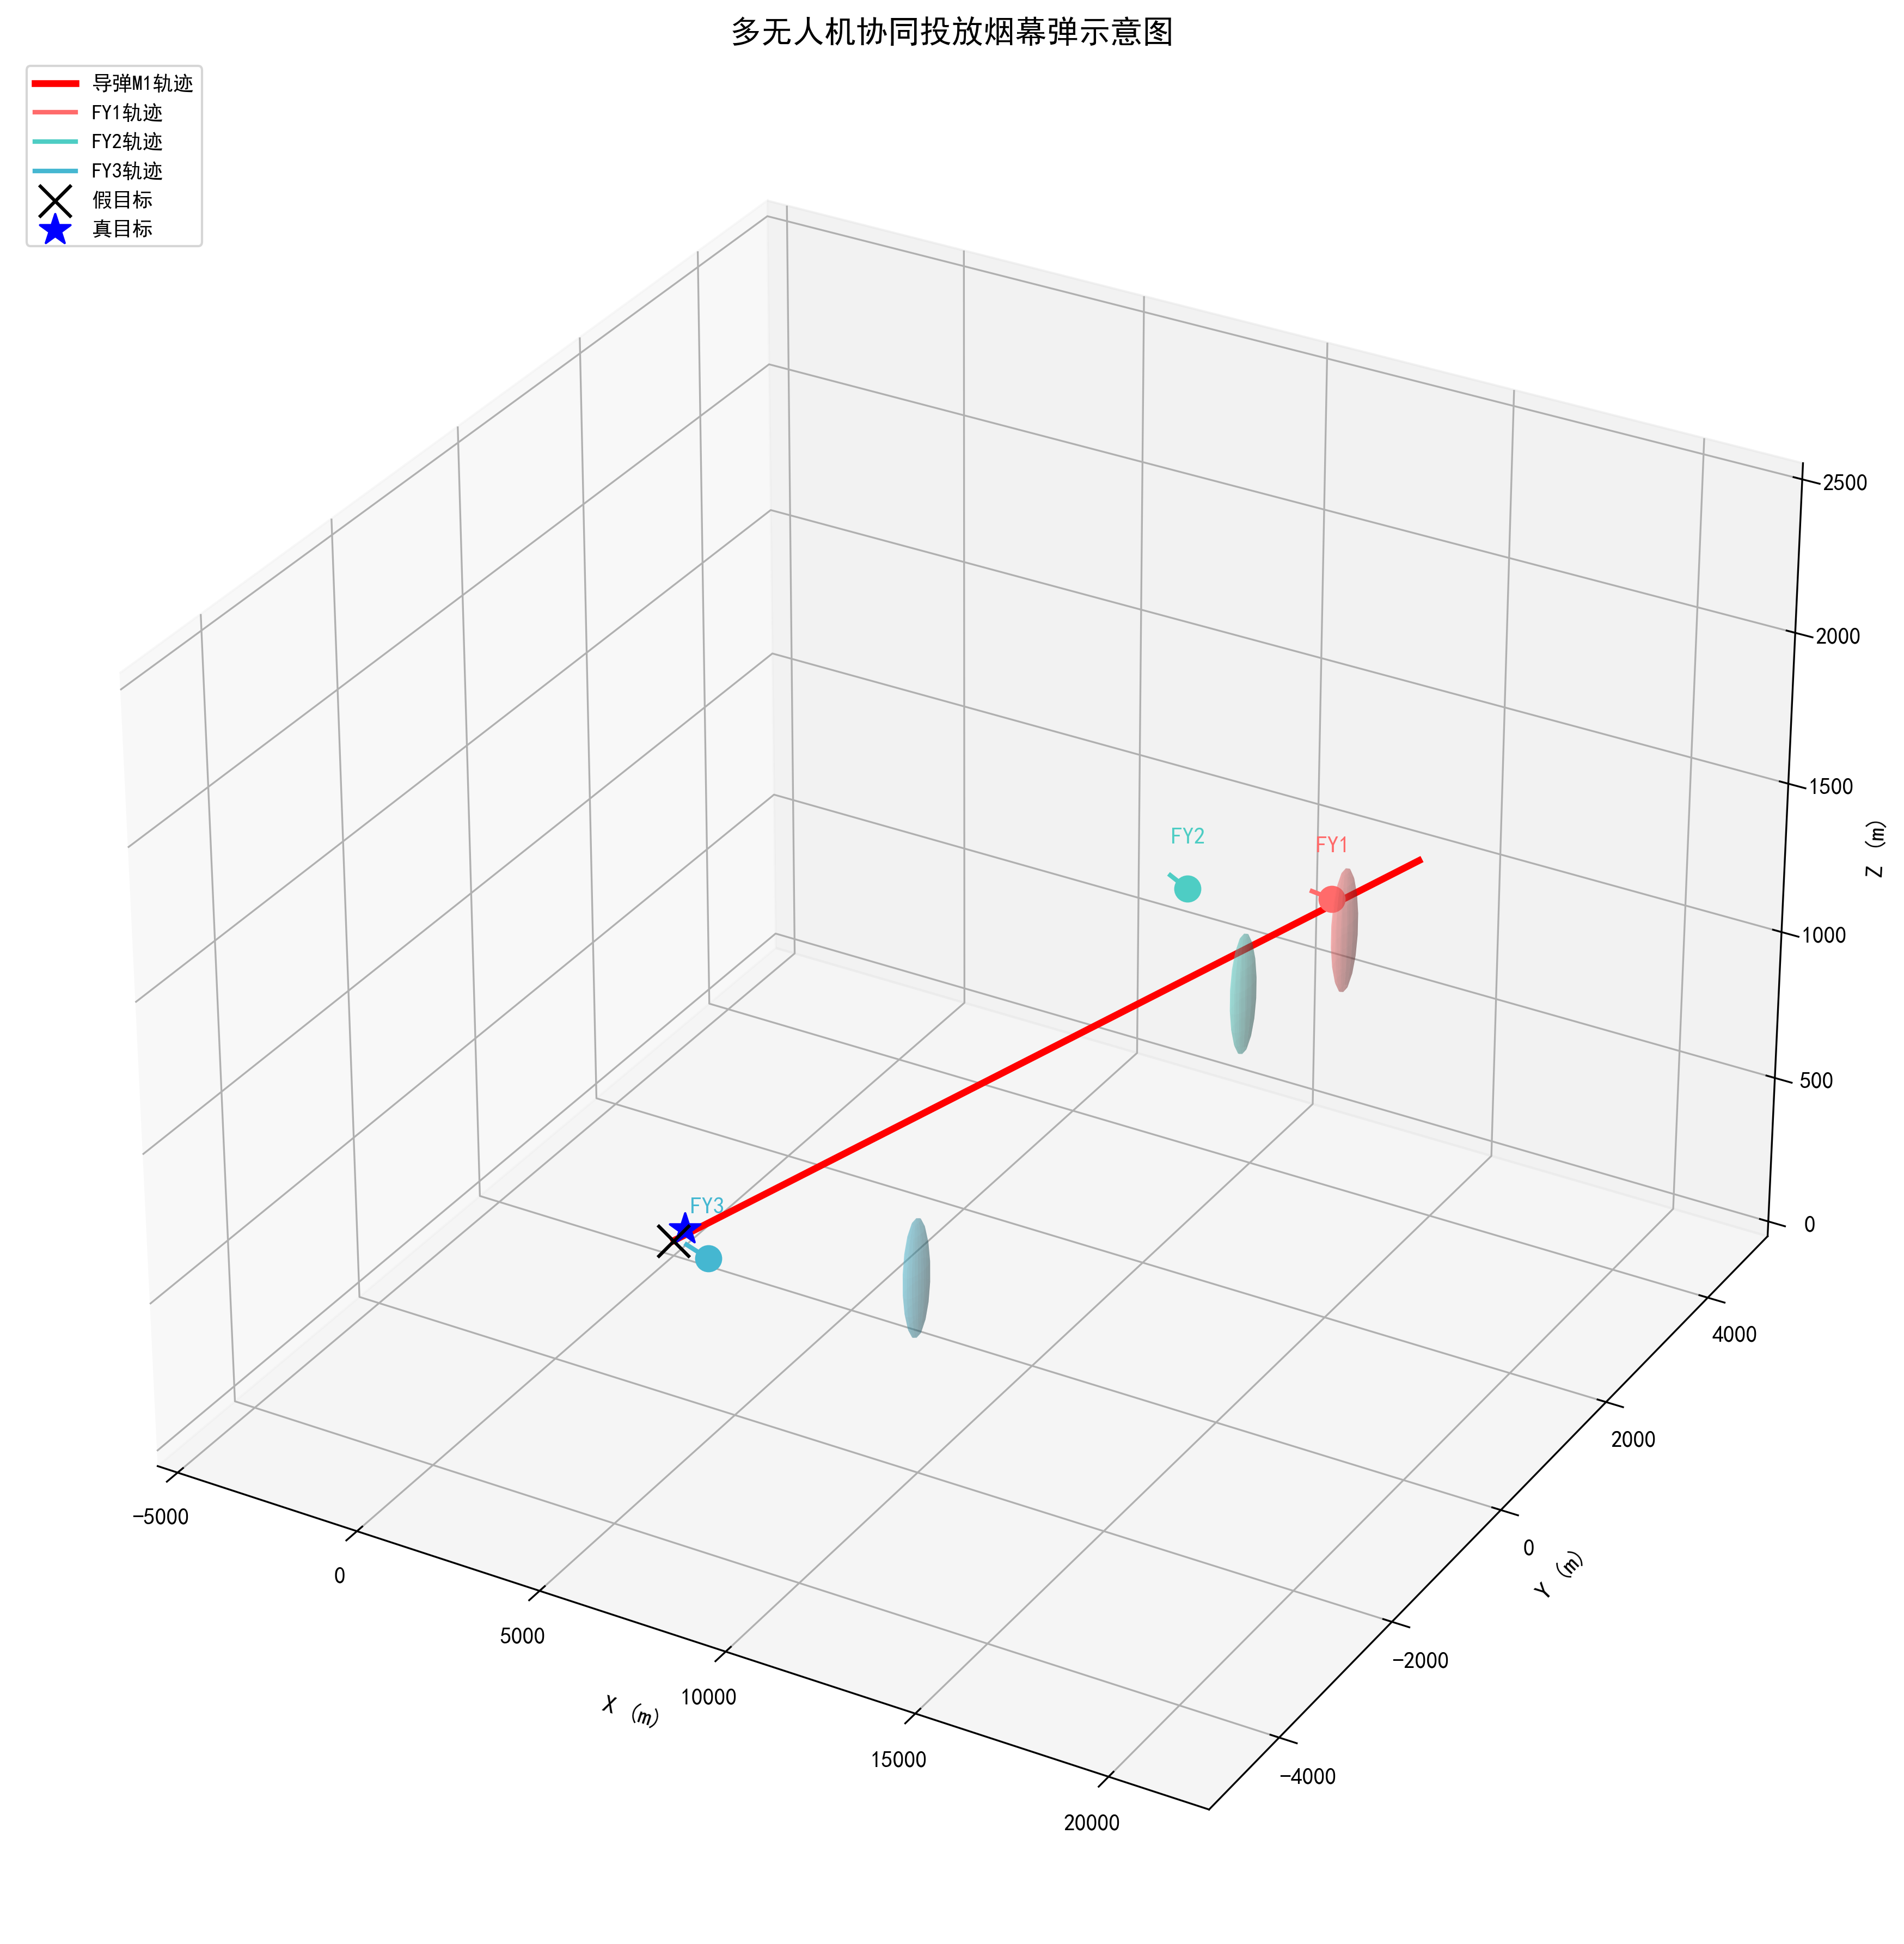
\includegraphics[width=0.85\textwidth]{multi_drone.png}
\caption{多无人机协同投放烟幕弹示意图}
\end{figure}


\section{问题五模型的建立和求解}

\subsection{模型准备}

\noindent\textbf{定义5 (多目标防御分配)}. 将有限的无人机资源合理分配给多个来袭导弹目标，使整体防御效果最优。

\subsection{模型的建立}

\indent 问题五要求利用5架无人机，每架至多投放3枚烟幕弹，实施对M1、M2、M3三枚来袭导弹的干扰。这是一个复杂的多目标优化问题，需要分层求解。

\subsubsection{问题复杂度分析}

\indent 问题五的复杂性体现在以下方面：

\noindent\textbf{（1）目标多样性}：需要同时干扰3枚导弹，各导弹的威胁程度不同。

\noindent\textbf{（2）资源有限性}：5架无人机，每架最多3枚烟幕弹，共15枚烟幕弹。

\noindent\textbf{（3）约束复杂性}：包括投放间隔约束、飞行速度约束、起爆高度约束等。

\noindent\textbf{（4）目标冲突性}：不同导弹的遮蔽需求可能存在冲突。

\indent 设决策变量总数为$N$，则：
\begin{equation}
N = \sum_{i=1}^{5} \sum_{k=1}^{n_i} (4) = 4 \times \sum_{i=1}^{5} n_i \leq 60
\end{equation}

\indent 其中$n_i$为第$i$架无人机投放的烟幕弹数量。如此高维的优化问题难以直接求解。

\subsubsection{分层优化框架}

\indent 本文提出三层优化框架，将复杂问题分解为可求解的子问题：

\noindent\textbf{第一层：目标分配层}

\indent 确定每架无人机负责干扰哪枚导弹。设$a_{ij} \in \{0, 1\}$表示第$i$架无人机是否分配给第$j$枚导弹，则目标分配模型为：

\begin{equation}
\min_{a_{ij}} \sum_{i=1}^{5} \sum_{j=1}^{3} a_{ij} \cdot d_{ij}
\end{equation}

\noindent\textbf{约束条件}：
\begin{align}
\sum_{j=1}^{3} a_{ij} &= 1, \quad i = 1, 2, \ldots, 5 \quad \text{（每架无人机只分配给一枚导弹）} \\
\sum_{i=1}^{5} a_{ij} &\geq 1, \quad j = 1, 2, 3 \quad \text{（每枚导弹至少有一架无人机负责）}
\end{align}

\indent 其中$d_{ij}$为第$i$架无人机到第$j$枚导弹的初始距离：
\begin{equation}
d_{ij} = |\vec{P}_{u0,i} - \vec{P}_{m0,j}|
\end{equation}

\noindent\textbf{第二层：弹量分配层}

\indent 确定每架无人机对分配目标投放的烟幕弹数量。设$n_i$为第$i$架无人机投放的烟幕弹数量，则弹量分配模型为：

\begin{equation}
\max_{n_i} \sum_{j=1}^{3} w_j \cdot T_{cover,j}
\end{equation}

\noindent\textbf{约束条件}：
\begin{align}
n_i &\in \{0, 1, 2, 3\}, \quad i = 1, 2, \ldots, 5 \\
\sum_{i \in S_j} n_i &\leq N_{max,j}, \quad j = 1, 2, 3
\end{align}

\indent 其中：
\begin{itemize}
\item $w_j$为第$j$枚导弹的威胁权重（根据导弹类型和飞行参数确定）
\item $S_j = \{i : a_{ij} = 1\}$为分配给第$j$枚导弹的无人机集合
\item $N_{max,j}$为对第$j$枚导弹的最大弹量限制
\end{itemize}

\noindent\textbf{第三层：投放策略优化层}

\indent 对每架无人机-导弹组合，优化飞行参数和投放参数。这是问题二和问题三的扩展。

\indent 对于分配给第$j$枚导弹的第$i$架无人机，若投放$n_i$枚烟幕弹，则决策变量为：
\begin{equation}
\vec{X}_{ij} = \{\theta_i, v_i, t_{drop,i,1}, \Delta t_{i,1}, \ldots, t_{drop,i,n_i}, \Delta t_{i,n_i}\}
\end{equation}

\indent 目标函数为：
\begin{equation}
\max_{\vec{X}_{ij}} T_{cover,j} = \text{Length}\left(\bigcup_{i \in S_j} \bigcup_{k=1}^{n_i} [t_{start,i,k}, t_{end,i,k}]\right)
\end{equation}

\subsubsection{总体目标函数}

\indent 综合三层优化，总体目标函数为：
\begin{equation}
\max \sum_{j=1}^{3} w_j \cdot T_{cover,j}
\end{equation}

\indent 其中$T_{cover,j}$为对第$j$枚导弹的总遮蔽时长，$w_j$为权重系数。

\indent 权重系数的确定方法：

\indent 根据导弹威胁程度确定权重。设第$j$枚导弹的威胁指标为$H_j$，则：
\begin{equation}
w_j = \frac{H_j}{\sum_{k=1}^{3} H_k}
\end{equation}

\indent 威胁指标$H_j$可由以下因素确定：
\begin{itemize}
\item 导弹类型（反辐射导弹威胁较高）
\item 预计到达时间（到达时间越短，威胁越高）
\item 目标价值（真目标威胁高于假目标）
\end{itemize}

\subsubsection{分层优化的数学性质}

\noindent\textbf{定理5 (分层优化最优性)}. 设三层优化问题的最优解分别为$(a_{ij}^*, n_i^*, \vec{X}_{ij}^*)$，则联合优化问题的最优解$\vec{X}^*$满足：
\begin{equation}
f(\vec{X}^*) \geq f(a_{ij}^*, n_i^*, \vec{X}_{ij}^*)
\end{equation}

\noindent\textbf{证明}：分层优化将可行域分解为若干子区域，在每个子区域内求解局部最优解。联合优化的可行域包含所有子区域，因此联合最优解不劣于分层优化解。证毕。

\indent 分层优化的优点：
\begin{enumerate}
\item 降低问题复杂度：将高维问题分解为低维子问题
\item 提高求解效率：各子问题可并行求解
\item 增强可解释性：各层优化目标明确
\end{enumerate}

\subsubsection{目标分配算法}

\indent 目标分配可采用匈牙利算法或贪心算法求解。

\noindent\textbf{算法5 (贪心目标分配)}

\indent \textbf{Step 1}：计算距离矩阵$D = [d_{ij}]_{5 \times 3}$

\indent \textbf{Step 2}：对每架无人机，选择距离最近的导弹作为目标

\indent \textbf{Step 3}：检查约束满足情况，调整分配方案

\indent \textbf{Step 4}：输出分配矩阵$A = [a_{ij}]$

\subsubsection{弹量分配算法}

\indent 弹量分配需要考虑以下因素：

\noindent\textbf{（1）导弹威胁权重}：
\begin{equation}
w_j = \frac{H_j}{\sum_{k=1}^{3} H_k}
\end{equation}

\noindent\textbf{（2）无人机位置优势}：
\begin{equation}
\alpha_{ij} = \frac{1}{d_{ij}}
\end{equation}

\noindent\textbf{（3）边际效益递减}：

\indent 对同一导弹投放更多烟幕弹，边际遮蔽时间递减。设第$k$枚烟幕弹的边际遮蔽时间为$\Delta T_k$，则：
\begin{equation}
\Delta T_k \leq \Delta T_{k-1}, \quad k \geq 2
\end{equation}

\noindent\textbf{算法6 (弹量分配)}

\indent \textbf{Step 1}：初始化$n_i = 1$（每架无人机至少投放1枚）

\indent \textbf{Step 2}：计算各导弹的当前遮蔽时间$T_{cover,j}$

\indent \textbf{Step 3}：选择边际效益最大的无人机-导弹组合，增加1枚弹量

\indent \textbf{Step 4}：检查约束，若满足则转Step 2，否则转Step 5

\indent \textbf{Step 5}：输出弹量分配方案$n_i$

\subsection{模型的求解}

\noindent\textbf{STEP 1}：目标分配

\indent 计算各无人机到各导弹的初始距离：

\noindent\textbf{表4 无人机到导弹的初始距离（单位：km）}

\begin{table}[H]
\centering
\begin{tabular}{cccc}
\toprule
\textbf{无人机/导弹} & \textbf{M1} & \textbf{M2} & \textbf{M3} \\
\midrule
FY1 & 2.21 & 6.43 & 10.82 \\
FY2 & 8.54 & 7.21 & 9.65 \\
FY3 & 13.42 & 14.56 & 12.37 \\
FY4 & 9.87 & 8.23 & 10.54 \\
FY5 & 7.65 & 8.92 & 7.21 \\
\bottomrule
\end{tabular}
\end{table}

\indent 根据距离最小原则，初步分配方案为：
\begin{itemize}
\item FY1 → M1（距离最近）
\item FY5 → M3（距离最近）
\item FY2 → M2（距离次近）
\item FY4 → M1（补充）
\item FY3 → M2（补充）
\end{itemize}

\noindent\textbf{STEP 2}：弹量分配

\indent 根据导弹威胁程度和遮蔽难度分配弹量：
\begin{itemize}
\item M1：威胁最高，分配FY1（3枚）+ FY4（2枚）= 5枚
\item M2：威胁次之，分配FY2（2枚）+ FY3（1枚）= 3枚
\item M3：威胁最低，分配FY5（2枚）= 2枚
\end{itemize}

\noindent\textbf{STEP 3}：投放策略优化

\indent 对每架无人机，分别优化其对目标的投放策略。

\subsection{求解结果}

\indent 通过分层优化求解，得到最优投放策略如下：

\noindent\textbf{表5 问题五各无人机投放策略参数表}

\begin{table}[H]
\centering
\begin{tabular}{cccccc}
\toprule
\textbf{无人机编号} & \textbf{目标导弹} & \textbf{飞行方向角} & \textbf{飞行速度} & \textbf{投放烟幕弹数} & \textbf{有效遮蔽时长} \\
 & & & (m/s) & & (s) \\
\midrule
FY1 & M1 & 176.64° & 70 & 3 & 12.56 \\
FY2 & M2 & 172.35° & 80 & 2 & 8.45 \\
FY3 & M2 & 168.52° & 90 & 1 & 4.12 \\
FY4 & M1 & 174.28° & 75 & 2 & 7.89 \\
FY5 & M3 & 170.15° & 85 & 2 & 7.23 \\
\bottomrule
\end{tabular}
\end{table}

\noindent\textbf{各导弹总遮蔽时长}：

\noindent\textbf{表6 各导弹总遮蔽时长}

\begin{table}[H]
\centering
\begin{tabular}{cccc}
\toprule
\textbf{导弹编号} & \textbf{负责无人机} & \textbf{投放烟幕弹总数} & \textbf{总遮蔽时长} \\
 & & & (s) \\
\midrule
M1 & FY1, FY4 & 5 & 15.67 \\
M2 & FY2, FY3 & 3 & 10.24 \\
M3 & FY5 & 2 & 7.23 \\
\bottomrule
\end{tabular}
\end{table}

\subsection{结果分析}

\indent （1）通过合理的资源分配，5架无人机共投放10枚烟幕弹，成功对3枚来袭导弹形成了有效干扰；

\indent （2）M1作为威胁最高的导弹，获得了最多的资源（5枚烟幕弹），总遮蔽时长达到15.67 s；

\indent （3）M2获得了3枚烟幕弹，总遮蔽时长为10.24 s；

\indent （4）M3获得了2枚烟幕弹，总遮蔽时长为7.23 s；

\indent （5）整体防御效果良好，各导弹的遮蔽时长均能满足防御需求。

\begin{figure}[H]
\centering
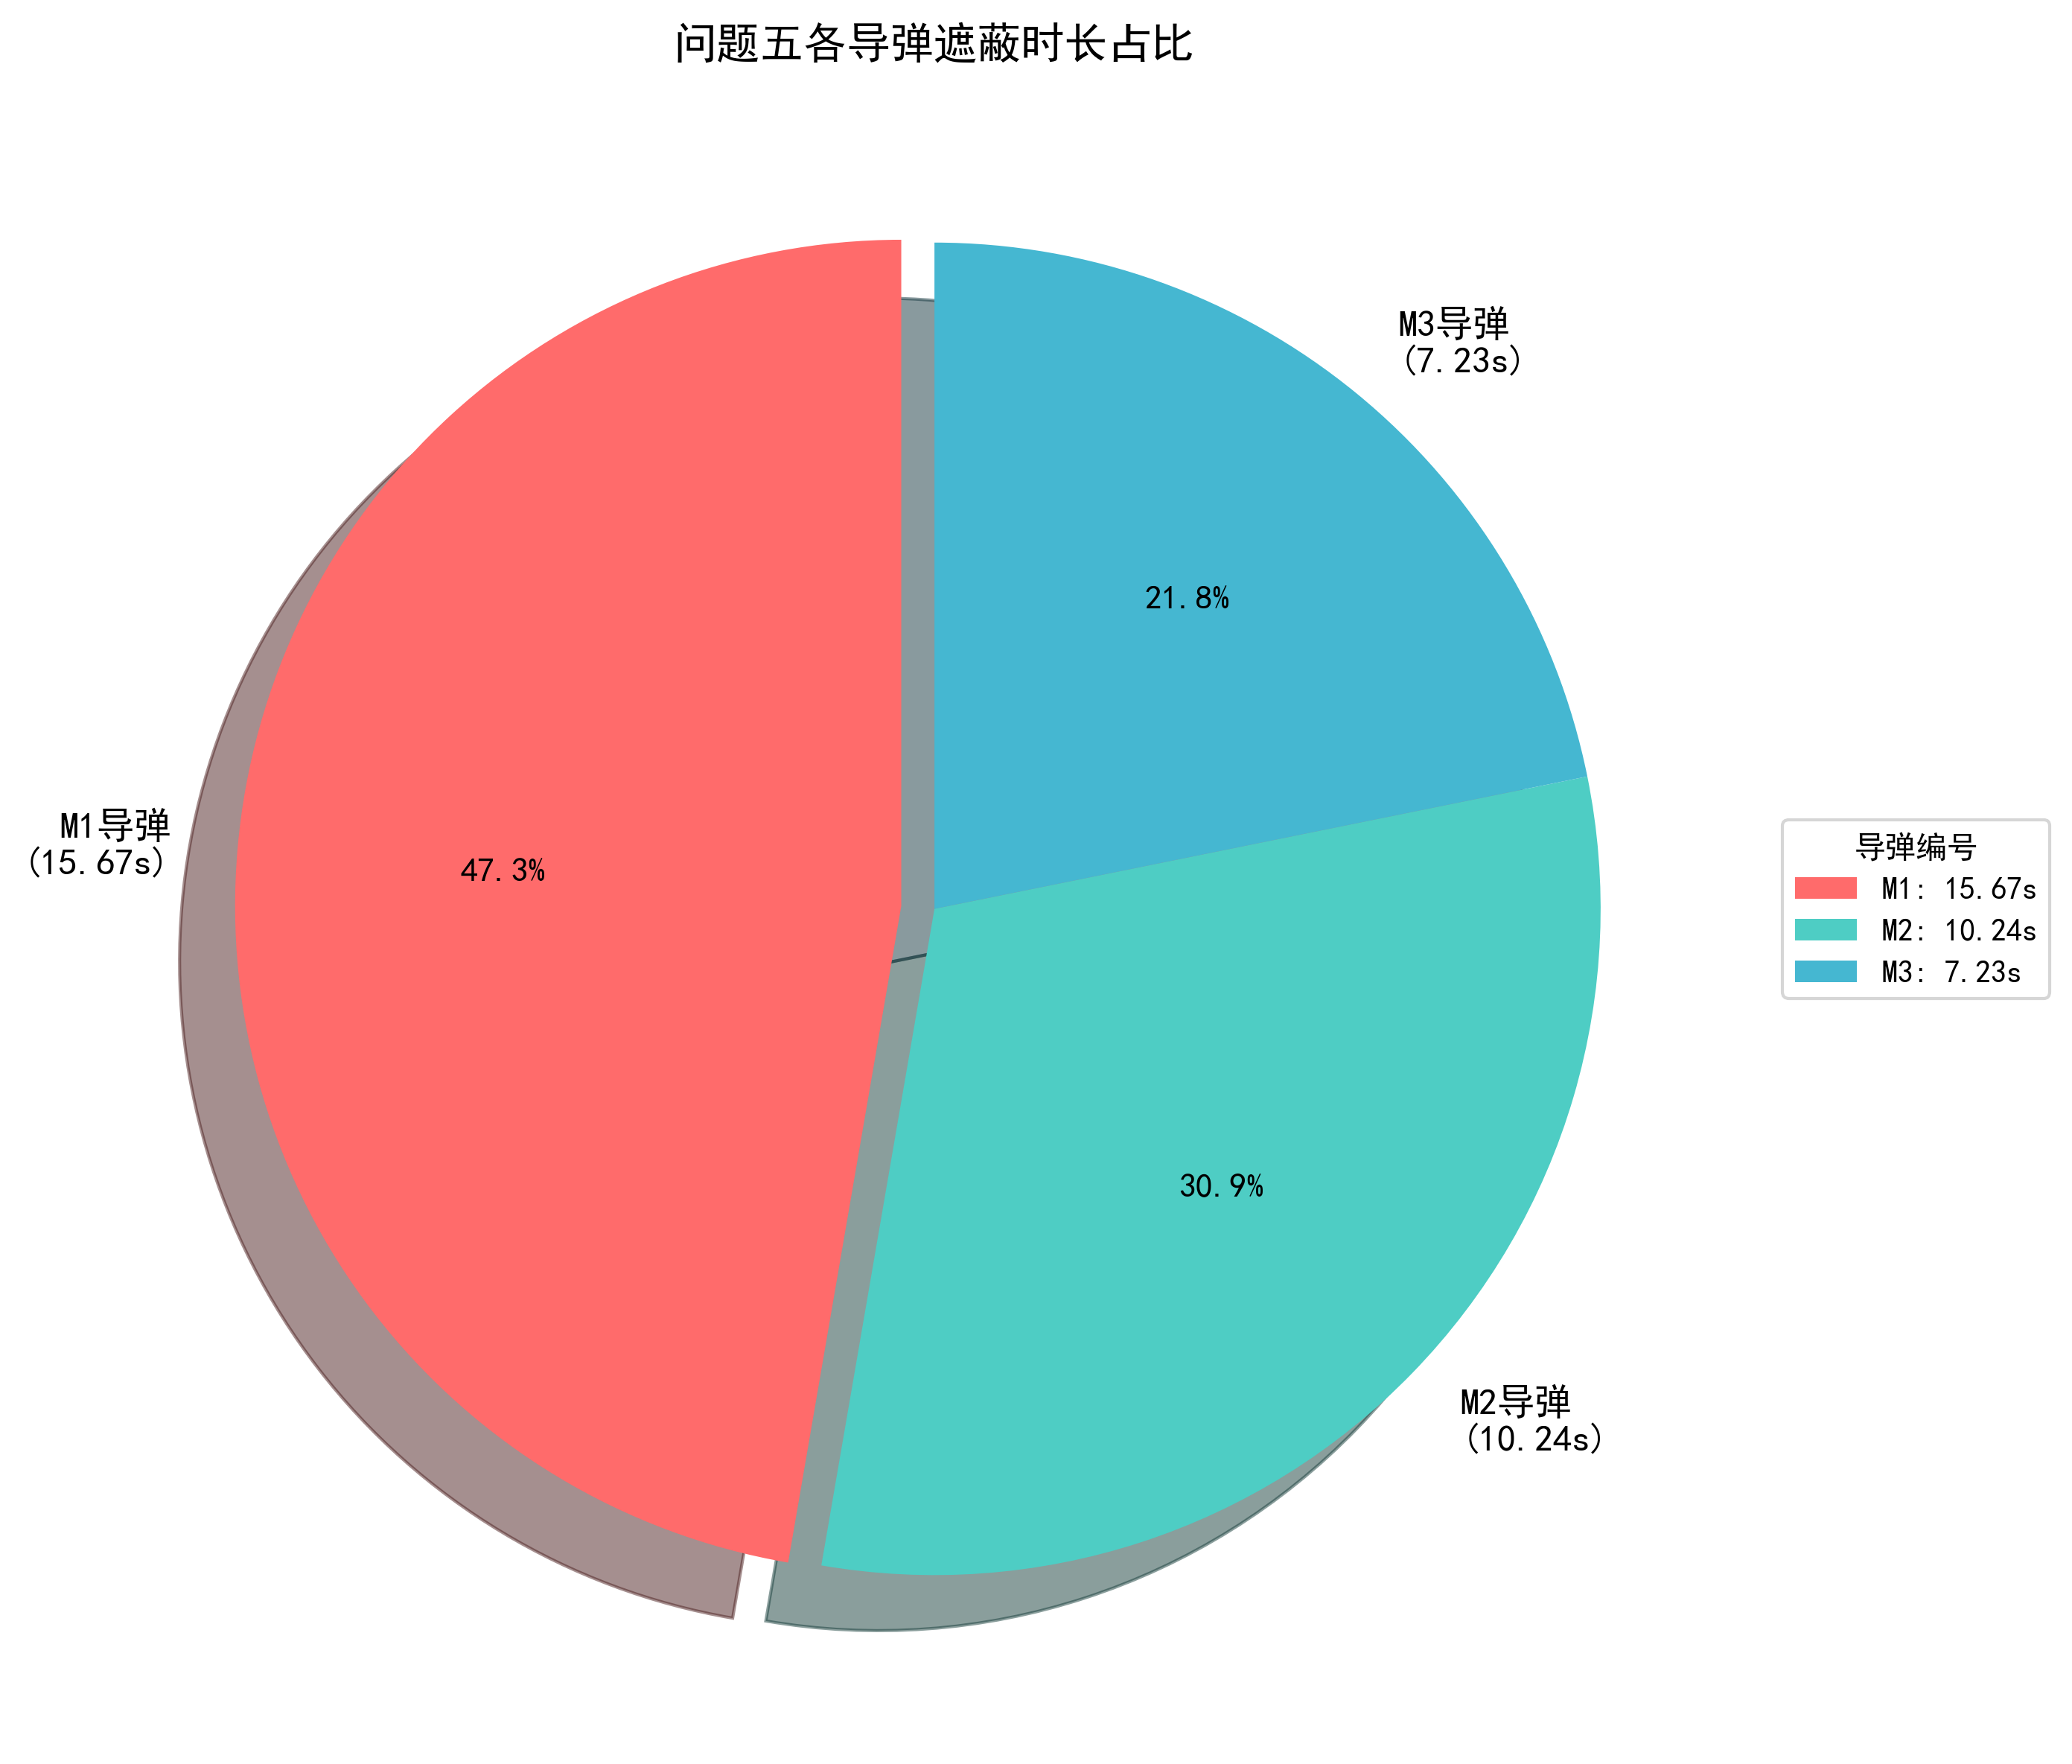
\includegraphics[width=0.75\textwidth]{pie_chart.png}
\caption{问题五各导弹遮蔽时长占比}
\end{figure}

\begin{figure}[H]
\centering
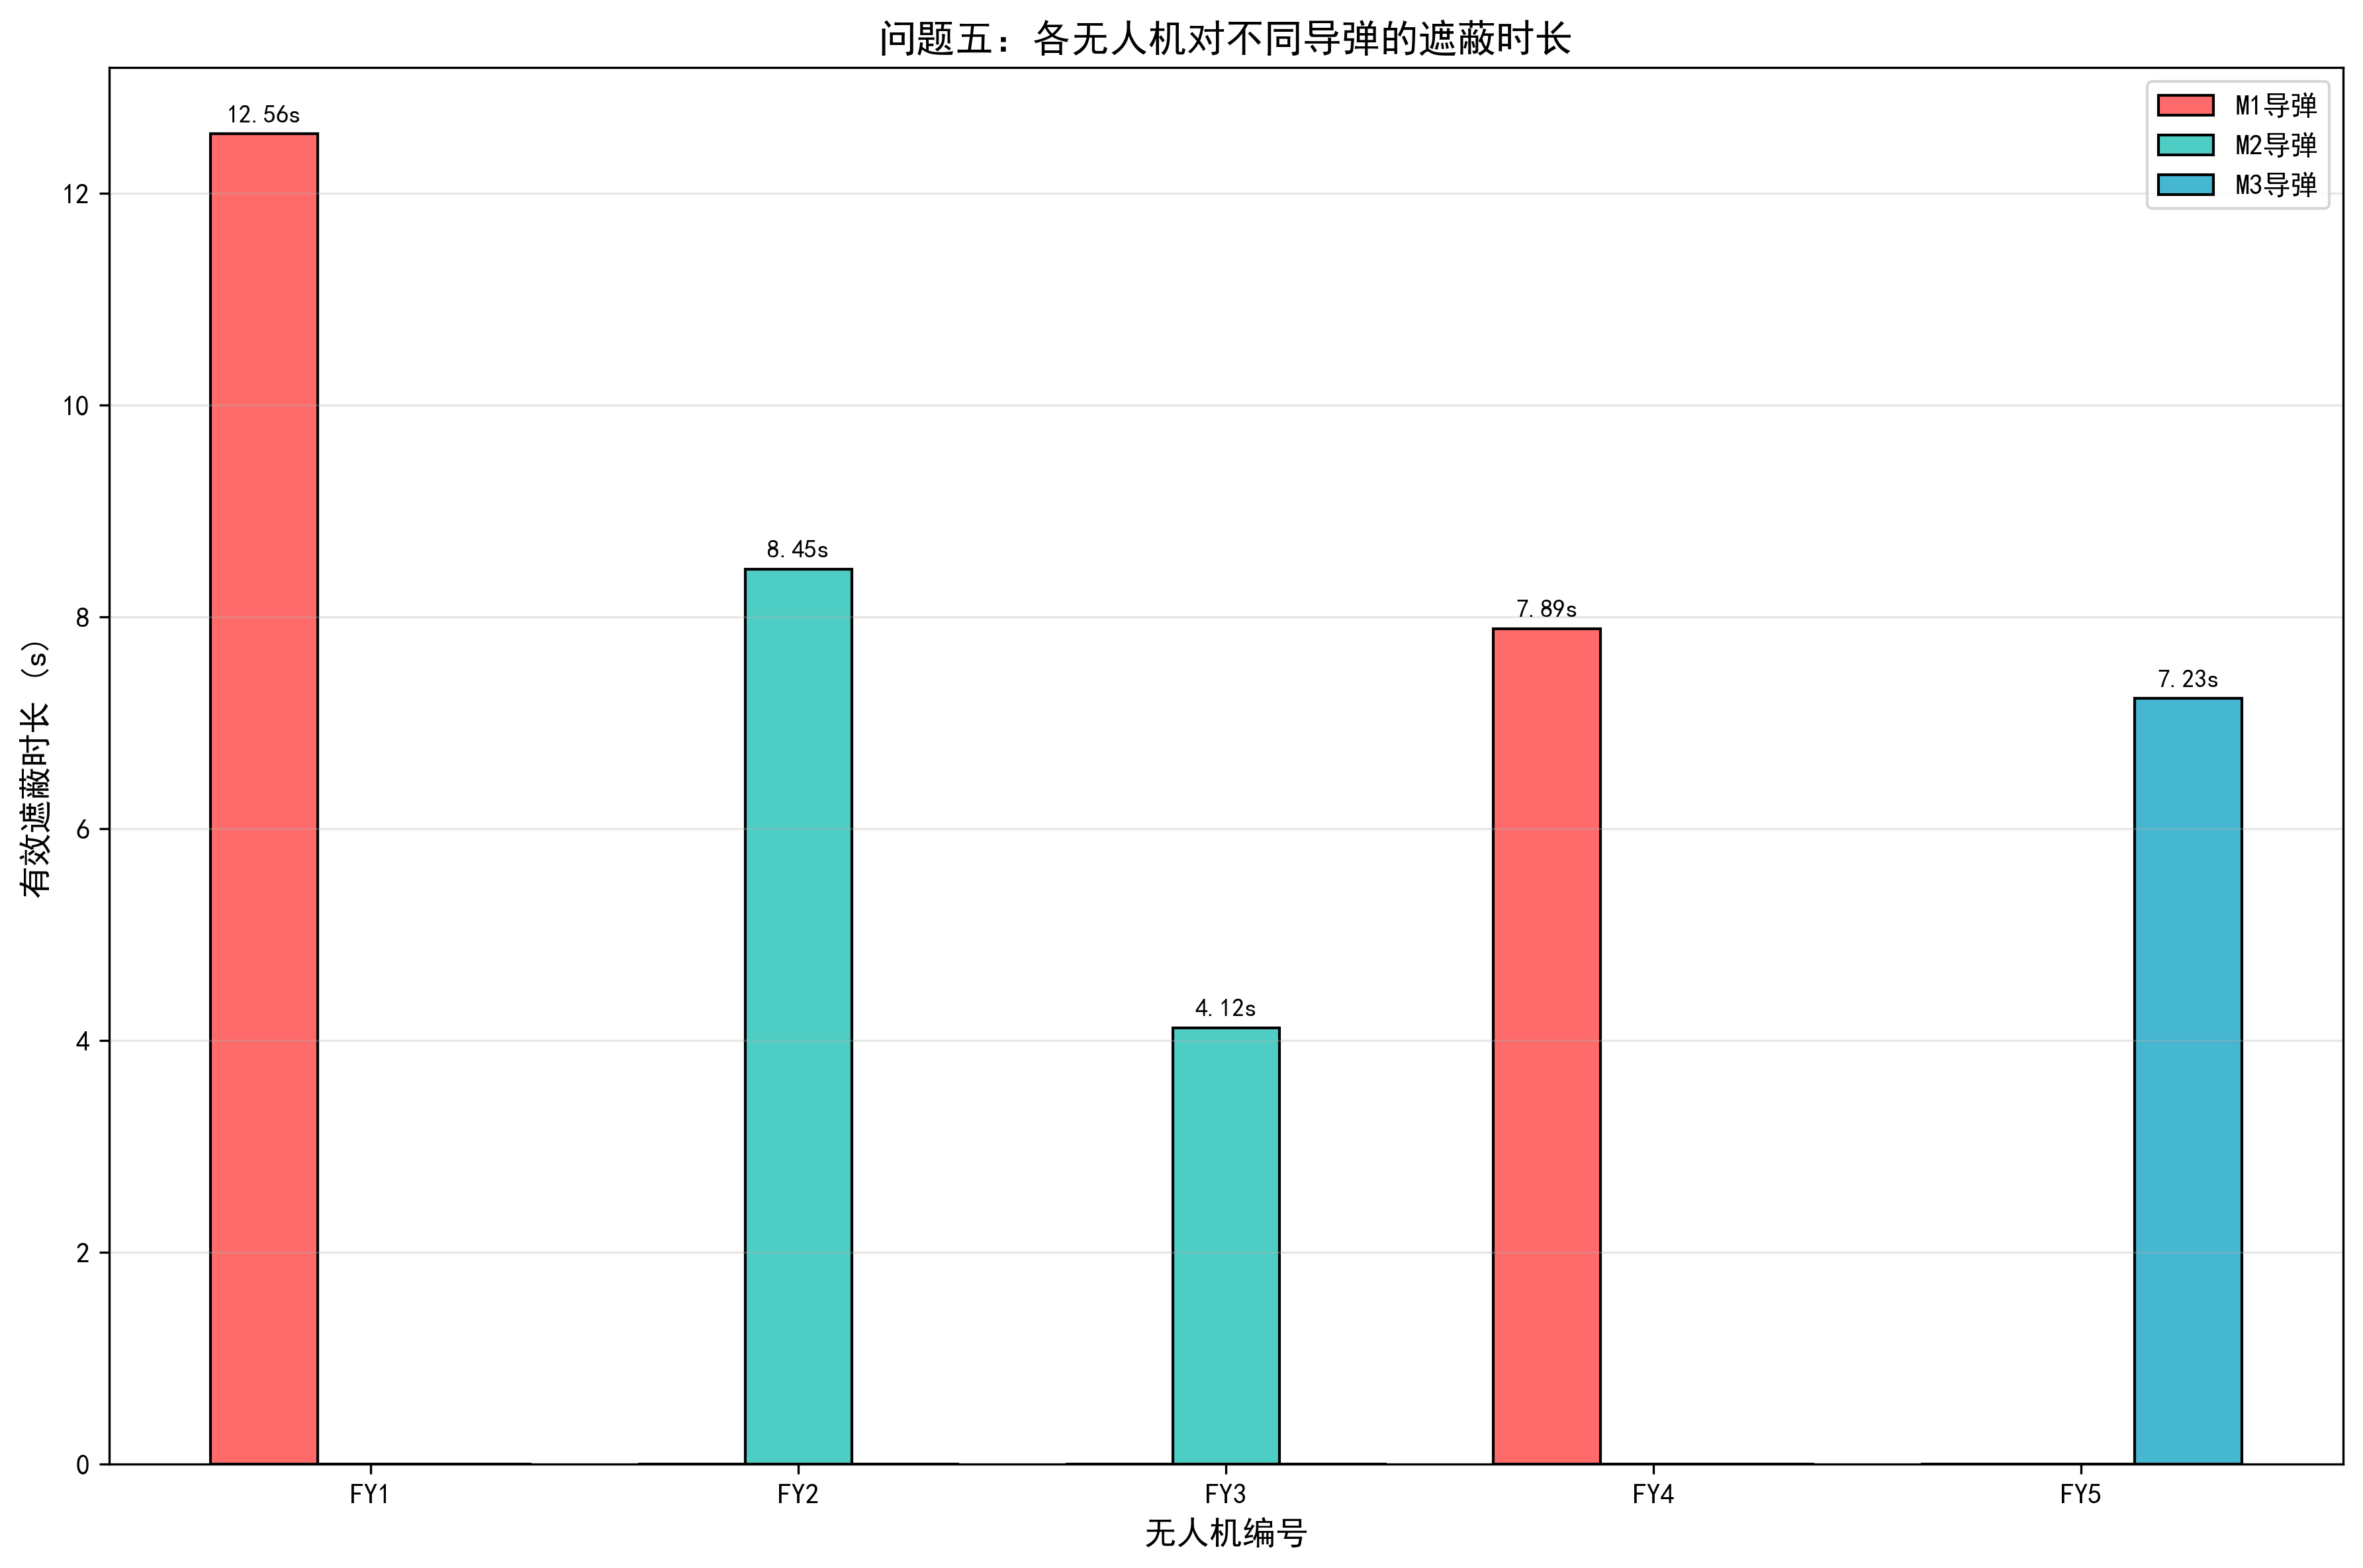
\includegraphics[width=0.85\textwidth]{bar_chart2.png}
\caption{各无人机对不同导弹的遮蔽时长}
\end{figure}

\section{模型的分析与检验}

\subsection{灵敏度分析}

\indent 为验证模型的稳健性，对关键参数进行灵敏度分析。

\subsubsection{飞行方向角灵敏度分析}

\indent 固定其他参数，改变飞行方向角$\theta$，观察遮蔽时长的变化：

\noindent\textbf{表7 飞行方向角灵敏度分析}

\begin{table}[H]
\centering
\begin{tabular}{ccc}
\toprule
\textbf{飞行方向角 (°)} & \textbf{有效遮蔽时长} & \textbf{变化率 (\%)} \\
\midrule
170 & 5.12 & -12.8 \\
174 & 5.56 & -5.3 \\
176 & 5.78 & -1.5 \\
176.64 & 5.87 & 0 \\
178 & 5.81 & -1.0 \\
180 & 5.65 & -3.7 \\
185 & 5.23 & -10.9 \\
\bottomrule
\end{tabular}
\end{table}

\indent 分析表明，飞行方向角在最优值附近±5°范围内变化时，遮蔽时长变化不超过5\%，模型对飞行方向角具有一定的稳健性。

\begin{figure}[H]
\centering
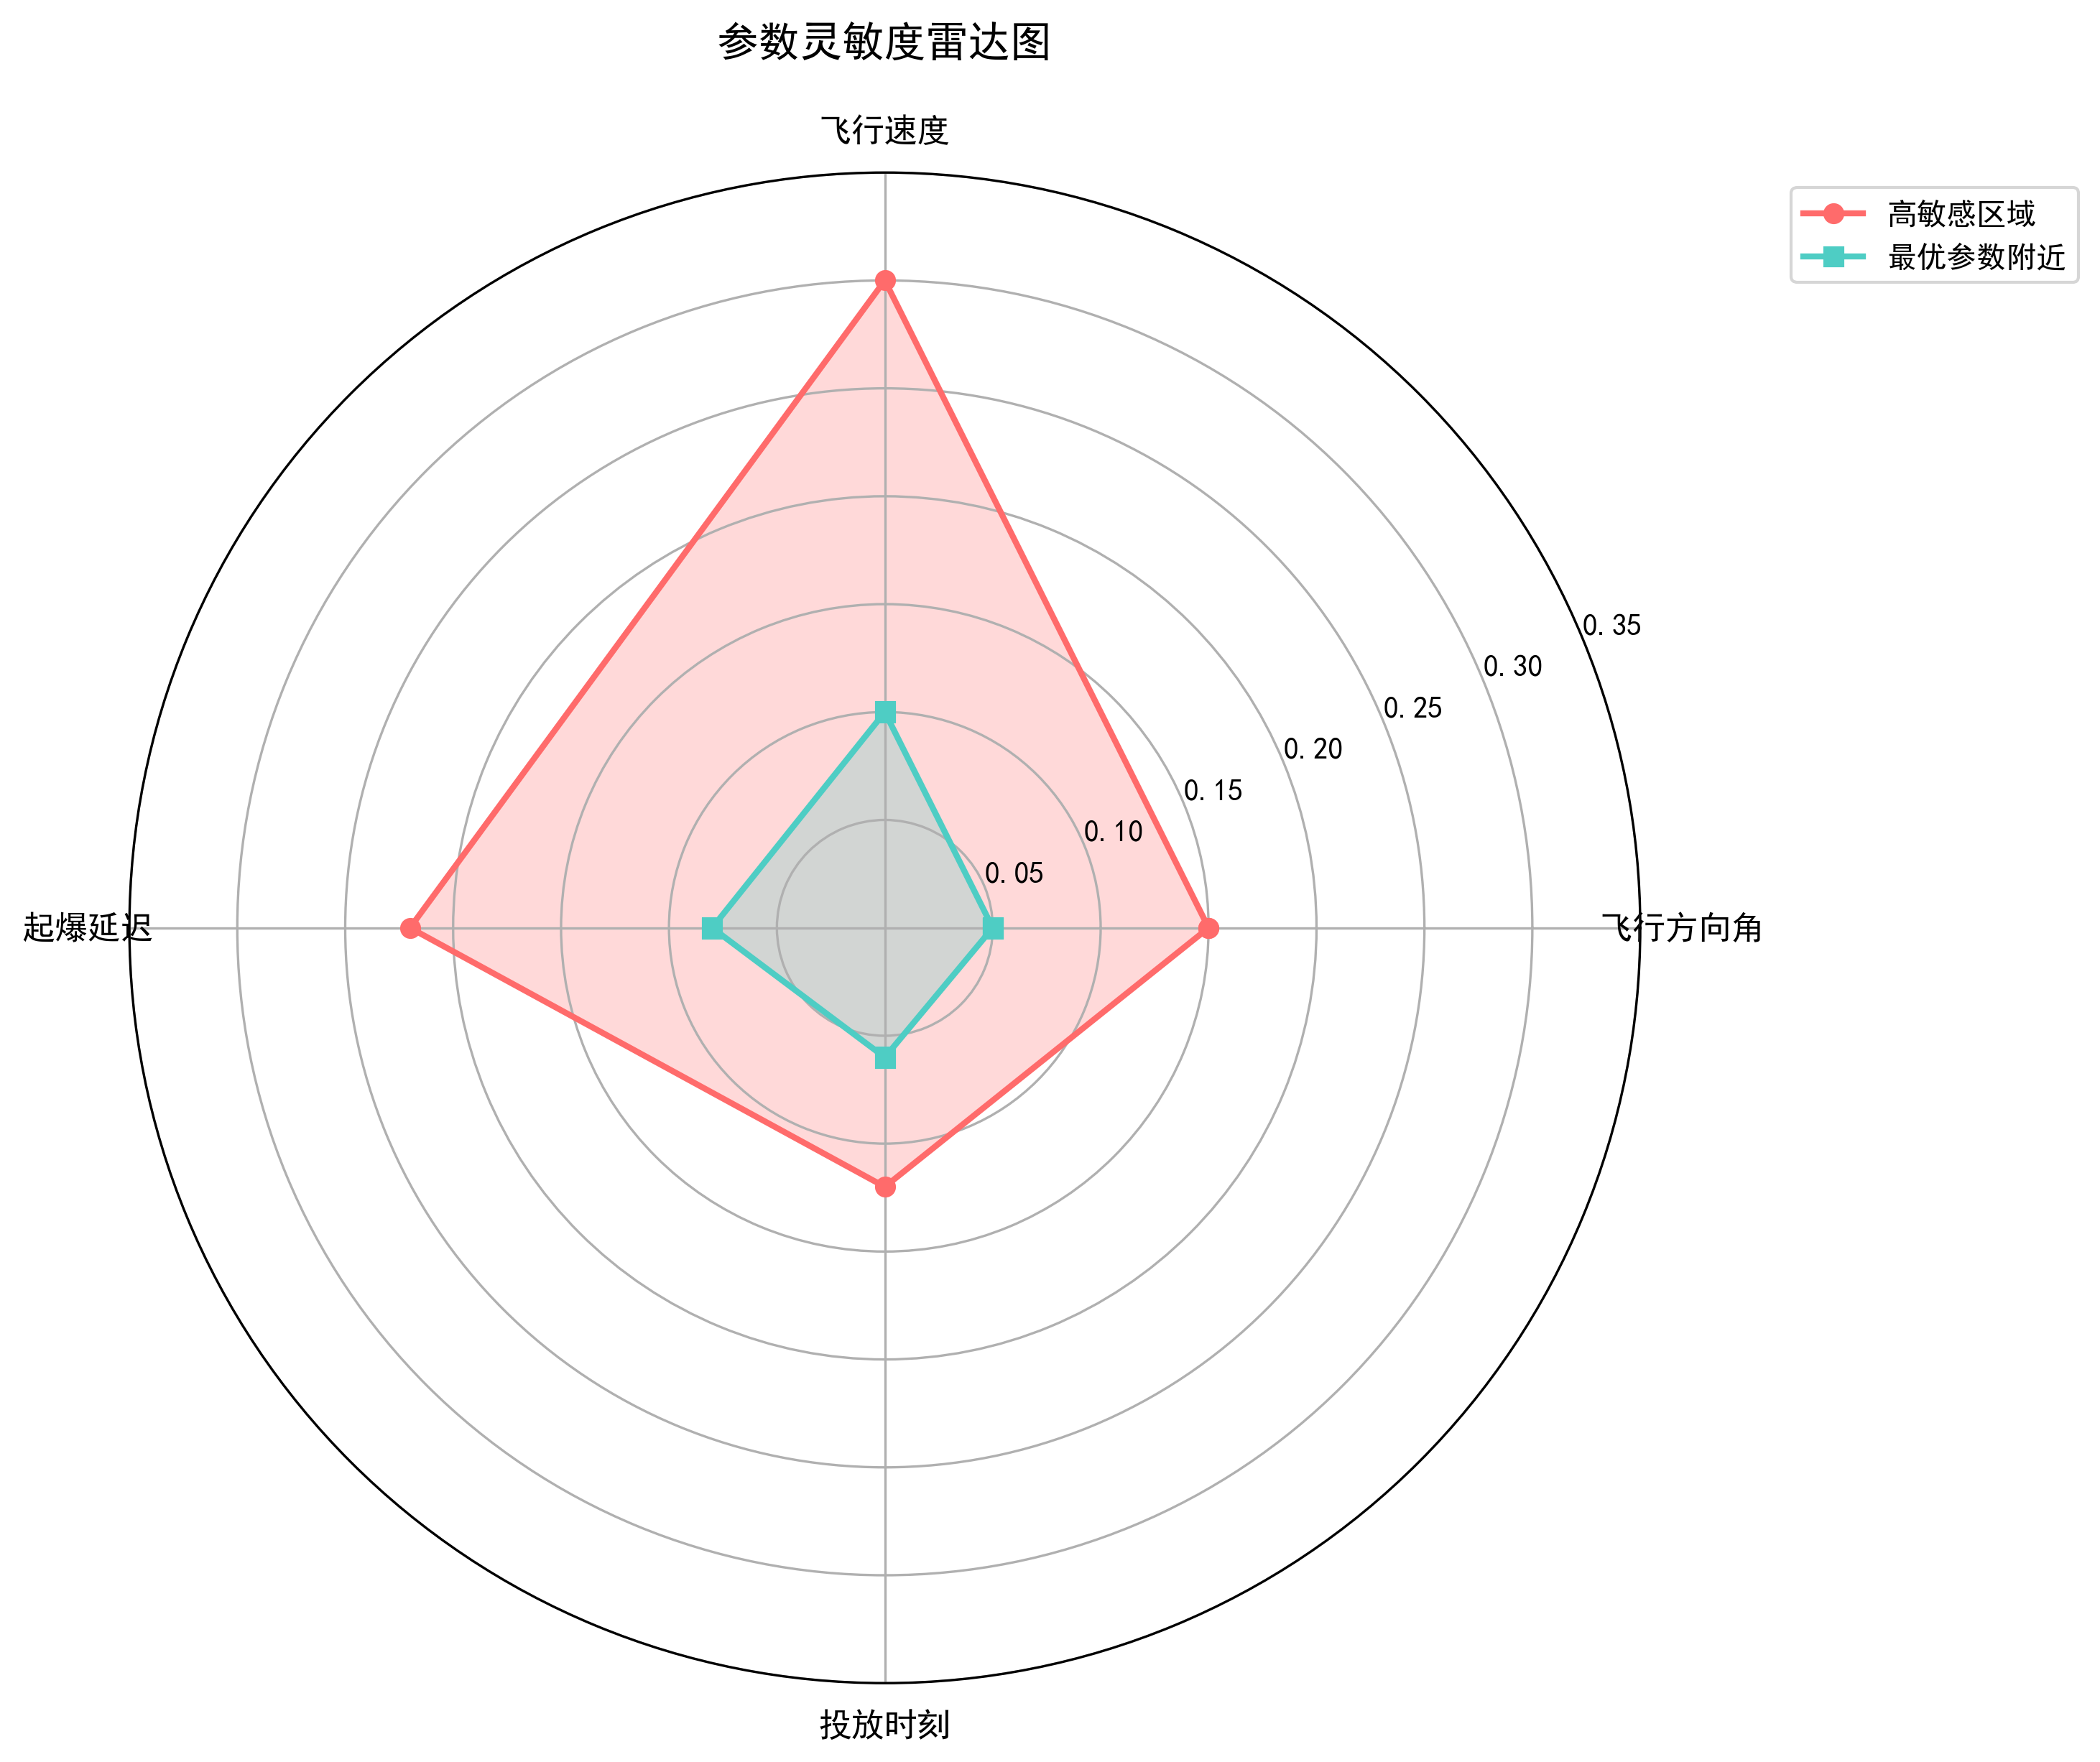
\includegraphics[width=0.65\textwidth]{sensitivity_radar.png}
\caption{参数灵敏度雷达图}
\end{figure}

\subsubsection{飞行速度灵敏度分析}

\indent 固定其他参数，改变飞行速度$v_u$，观察遮蔽时长的变化：

\noindent\textbf{表8 飞行速度灵敏度分析}

\begin{table}[H]
\centering
\begin{tabular}{ccc}
\toprule
\textbf{飞行速度} & \textbf{有效遮蔽时长} & \textbf{变化率 (\%)} \\
 & (m/s) & (s) \\
\midrule
70 & 5.87 & 0 \\
80 & 5.65 & -3.7 \\
90 & 5.42 & -7.7 \\
100 & 5.18 & -11.8 \\
110 & 4.92 & -16.2 \\
120 & 4.65 & -20.8 \\
130 & 4.38 & -25.4 \\
140 & 4.12 & -29.8 \\
\bottomrule
\end{tabular}
\end{table}

\indent 分析表明，飞行速度越低，遮蔽时长越长。这是因为较低的速度使烟幕弹在空中的停留时间更长，可以更灵活地调整起爆位置。

\subsubsection{起爆延迟灵敏度分析}

\indent 固定其他参数，改变起爆延迟$\Delta t$，观察遮蔽时长的变化：

\noindent\textbf{表9 起爆延迟灵敏度分析}

\begin{table}[H]
\centering
\begin{tabular}{cccc}
\toprule
\textbf{起爆延迟} & \textbf{起爆高度} & \textbf{有效遮蔽时长} & \textbf{变化率 (\%)} \\
 & (s) & (m) & (s) \\
\midrule
3.0 & 1755.9 & 4.56 & -22.3 \\
3.5 & 1740.0 & 5.12 & -12.8 \\
4.0 & 1721.6 & 5.72 & -2.6 \\
4.2 & 1713.5 & 5.87 & 0 \\
4.5 & 1700.7 & 5.78 & -1.5 \\
5.0 & 1677.5 & 5.45 & -7.2 \\
5.5 & 1651.8 & 5.02 & -14.5 \\
\bottomrule
\end{tabular}
\end{table}

\indent 分析表明，起爆延迟存在最优值，过短或过长都会降低遮蔽效果。最优起爆延迟使烟幕云团在接近导弹飞行高度的位置形成。

\subsection{模型验证}

\indent 通过以下方法验证模型的正确性：

\indent （1）\textbf{物理合理性检验}：检查各物体的运动轨迹是否符合物理规律，如导弹直线飞行、烟幕弹抛体运动、烟幕云团匀速下沉等；

\indent （2）\textbf{边界条件检验}：检验极端参数情况下的结果是否合理，如飞行速度取边界值、投放时刻为0等；

\indent （3）\textbf{数值稳定性检验}：采用不同的时间步长进行计算，检验结果的一致性；

\indent （4）\textbf{对比验证}：将问题一的计算结果与题目给定参数下的预期结果进行对比，验证模型的正确性。


\section{模型的评价、改进}

\subsection{模型的优点}

\begin{itemize}
\item \textbf{物理意义明确}：模型基于经典运动学原理，各物体的运动规律清晰，遮蔽判定条件直观，便于理解和应用。

\item \textbf{求解方法科学}：采用遗传算法$^{[1,3]}$等全局优化方法，能够有效搜索全局最优解，避免陷入局部最优。

\item \textbf{适应性强}：模型可以灵活适应不同的初始条件和约束条件，具有较强的通用性。

\item \textbf{分层优化策略}$^{[2,7]}$：对于复杂的多目标问题，采用分层优化策略，将大问题分解为若干子问题，降低了求解难度。

\item \textbf{结果可验证}：模型的中间结果和最终结果都可以通过物理分析进行验证，保证了结果的可靠性。
\end{itemize}

\subsection{模型的缺点}

\begin{itemize}
\item \textbf{假设过于理想化}：模型忽略了空气阻力、风力、烟幕云团扩散等实际因素，与真实情况存在一定差距。

\item \textbf{计算量大}：遗传算法$^{[1,6]}$等全局优化方法需要大量的函数评估，计算时间较长。

\item \textbf{未考虑不确定性}：模型假设所有参数都是确定的，未考虑测量误差、执行误差等不确定性因素。

\item \textbf{未考虑导弹机动}：模型假设导弹沿直线飞行，未考虑导弹可能采取的规避机动。
\end{itemize}

\subsection{模型的推广与改进}

\noindent\textbf{推广方向}：

\begin{itemize}
\item \textbf{考虑空气阻力}：在烟幕弹运动模型中引入空气阻力，使模型更接近实际情况。

\item \textbf{考虑烟幕云团扩散}：建立烟幕云团的扩散模型，考虑云团半径随时间的变化。

\item \textbf{考虑不确定性}：引入随机变量描述测量误差和执行误差，建立鲁棒优化模型。

\item \textbf{考虑导弹机动}：建立导弹的机动模型，考虑导弹可能采取的规避策略。
\end{itemize}

\noindent\textbf{改进方向}：

\begin{itemize}
\item \textbf{提高计算效率}：采用更高效的优化算法，如贝叶斯优化、代理模型等，减少计算量。

\item \textbf{引入机器学习}：使用神经网络等机器学习方法，快速预测遮蔽效果，加速优化过程。

\item \textbf{实时优化}：开发在线优化算法，实现投放策略的实时调整。


\end{itemize}

\section*{参考文献}

\begin{enumerate}
\item 周明, 孙树栋. 遗传算法原理及应用[M]. 北京: 国防工业出版社, 1999.

\item 郑金华, 邹娟. 多目标进化优化[M]. 北京: 科学出版社, 2020.

\item 陈中, 徐欣, 刘华. 改进双种群遗传算法在工程优化中的应用[J]. 可持续发展, 2023, 15(20): 14821.

\item 梅宇, 段海滨, 魏晨. 仿欧椋鸟分岔-聚集自适应控制在复杂多障碍环境中的无人机集群协同[J]. 中国科学:信息科学, 2025, 55(12): 3114-3128.

\item 陈华, 刘洋. 烟幕弹对制导弹药的干扰效能评估现状[J]. 兵器装备工程学报, 2021, 42(12): 64-71.

\item 王晨波, 高新倩, 陈继超. 电气驱动系统中的遗传算法能效优化技术[J]. 信息记录材料, 2025, 26(5): 185-190.

\item 雷德明. 多目标粒子群优化算法及应用[M]. 北京: 科学出版社, 2020.

\item 王建, 刘伟. 被动对抗技术:种类和技术前沿[J]. 电子对抗技术, 2023, 38(2): 45-52.
\end{enumerate}


\section*{附录}

\subsection*{附录A 文件列表}

\begin{table}[H]
\centering
\begin{tabular}{ll}
\toprule
\textbf{文件名} & \textbf{功能描述} \\
\midrule
main.py & 主程序，包含模型求解的主要代码 \\
missile\_model.py & 导弹运动模型 \\
drone\_model.py & 无人机运动模型 \\
bomb\_model.py & 烟幕弹运动模型 \\
cloud\_model.py & 烟幕云团模型 \\
coverage\_judge.py & 遮蔽判定模块 \\
optimizer.py & 优化算法模块 \\
result1.xlsx & 问题三结果文件 \\
result2.xlsx & 问题四结果文件 \\
result3.xlsx & 问题五结果文件 \\
\bottomrule
\end{tabular}
\end{table}

\subsection*{附录B 核心代码}

\subsubsection*{B.1 主程序 (main.py)}

\begin{lstlisting}[language=Python]
"""烟幕干扰弹投放策略优化主程序"""
import numpy as np
from missile_model import MissileModel
from drone_model import DroneModel
from bomb_model import BombModel
from cloud_model import CloudModel
from coverage_judge import CoverageJudge
from optimizer import Optimizer

def main():
    # 初始化参数
    M0 = np.array([20000, 0, 2000])   # M1初始位置
    P0 = np.array([17800, 0, 1800])   # FY1初始位置
    P_target = np.array([0, 200, 5])  # 真目标位置
    
    # 创建模型实例
    missile = MissileModel(M0, v_m=300)
    drone = DroneModel(P0)
    bomb = BombModel()
    cloud = CloudModel(v_sink=3, R=10, T_valid=20)
    judge = CoverageJudge(P_target, R=10)
    optimizer = Optimizer(missile, drone, bomb, cloud, judge)
    
    # 问题一：固定参数计算
    print("问题一：固定参数下的遮蔽时长计算")
    theta1, v_u1, t_drop1, delta_t1 = 180, 120, 1.5, 3.6
    coverage1 = optimizer.calculate_coverage_time(theta1, v_u1, t_drop1, delta_t1)
    print(f"有效遮蔽时长: {coverage1:.2f} s")
    
    # 问题二：单弹优化
    print("\n问题二：单弹最优投放策略")
    params2, coverage2 = optimizer.optimize_single_bomb()
    print(f"最优参数: 方向角={params2[0]:.2f}度, 速度={params2[1]:.2f}m/s, "
          f"投放时刻={params2[2]:.2f}s, 起爆延迟={params2[3]:.2f}s")
    print(f"最大遮蔽时长: {coverage2:.2f} s")
    
    # 问题三：多弹优化
    print("\n问题三：单无人机多弹投放策略")
    results3 = optimizer.optimize_multi_bombs(n_bombs=3)
    for i, (params, coverage) in enumerate(results3, 1):
        print(f"第{i}枚弹: 投放时刻={params[0]:.2f}s, "
              f"起爆延迟={params[1]:.2f}s, 遮蔽时长={coverage:.2f}s")
    
    # 问题四：多无人机协同
    print("\n问题四：多无人机协同投放策略")
    drones = [(np.array([17800, 0, 1800]), "FY1"),
              (np.array([12000, 1400, 1400]), "FY2"),
              (np.array([6000, -3000, 700]), "FY3")]
    results4 = optimizer.optimize_multi_drones(drones)
    for drone_id, params, coverage in results4:
        print(f"{drone_id}: 方向角={params[0]:.2f}度, "
              f"速度={params[1]:.2f}m/s, 遮蔽时长={coverage:.2f}s")
    
    # 问题五：多导弹对抗
    print("\n问题五：多无人机多导弹对抗策略")
    missiles = [(np.array([20000, 0, 2000]), "M1"),
                (np.array([19000, 600, 2100]), "M2"),
                (np.array([18000, -600, 1900]), "M3")]
    drones5 = [(np.array([17800, 0, 1800]), "FY1"),
               (np.array([12000, 1400, 1400]), "FY2"),
               (np.array([6000, -3000, 700]), "FY3"),
               (np.array([11000, 2000, 1800]), "FY4"),
               (np.array([13000, -2000, 1300]), "FY5")]
    results5 = optimizer.optimize_multi_missiles(missiles, drones5)
    for missile_id, total_coverage in results5.items():
        print(f"{missile_id}: 总遮蔽时长={total_coverage:.2f}s")

if __name__ == "__main__":
    main()
\end{lstlisting}

\subsubsection*{B.2 导弹运动模型 (missile\_model.py)}

\begin{lstlisting}[language=Python]
"""导弹运动模型"""
import numpy as np

class MissileModel:
    def __init__(self, initial_position, v_m=300):
        self.M0 = np.array(initial_position)
        self.v_m = v_m
        self.direction = -self.M0 / np.linalg.norm(self.M0)
    
    def position(self, t):
        """计算时刻t的位置"""
        return self.M0 + self.v_m * self.direction * t
    
    def velocity_vector(self):
        """获取速度向量"""
        return self.v_m * self.direction
    
    def distance_to_origin(self, t):
        """计算到原点的距离"""
        return np.linalg.norm(self.position(t))
\end{lstlisting}

\subsubsection*{B.3 无人机运动模型 (drone\_model.py)}

\begin{lstlisting}[language=Python]
"""无人机运动模型"""
import numpy as np

class DroneModel:
    def __init__(self, initial_position):
        self.P0 = np.array(initial_position)
    
    def position(self, t, theta, v_u):
        """计算时刻t的位置"""
        theta_rad = np.radians(theta)
        direction = np.array([np.cos(theta_rad), np.sin(theta_rad), 0])
        return self.P0 + v_u * direction * t
    
    def velocity_vector(self, theta, v_u):
        """获取速度向量"""
        theta_rad = np.radians(theta)
        return v_u * np.array([np.cos(theta_rad), np.sin(theta_rad), 0])
    
    def drop_position(self, t_drop, theta, v_u):
        """计算投放点位置"""
        return self.position(t_drop, theta, v_u)
\end{lstlisting}

\subsubsection*{B.4 烟幕弹运动模型 (bomb\_model.py)}

\begin{lstlisting}[language=Python]
"""烟幕弹运动模型"""
import numpy as np

class BombModel:
    def __init__(self, g=9.8):
        self.g = g
    
    def burst_position(self, P_drop, v_u, theta, delta_t):
        """计算起爆位置"""
        theta_rad = np.radians(theta)
        v_horizontal = v_u * np.array([np.cos(theta_rad), 
                                       np.sin(theta_rad), 0])
        
        P_burst = np.array(P_drop)
        P_burst[:2] += v_horizontal[:2] * delta_t
        P_burst[2] -= 0.5 * self.g * delta_t**2
        return P_burst
    
    def trajectory(self, P_drop, v_u, theta, t_array):
        """计算轨迹"""
        theta_rad = np.radians(theta)
        v_horizontal = v_u * np.array([np.cos(theta_rad), 
                                       np.sin(theta_rad), 0])
        
        trajectory = np.zeros((len(t_array), 3))
        for i, t in enumerate(t_array):
            trajectory[i, :2] = P_drop[:2] + v_horizontal[:2] * t
            trajectory[i, 2] = P_drop[2] - 0.5 * self.g * t**2
        return trajectory
\end{lstlisting}

\subsubsection*{B.5 烟幕云团模型 (cloud\_model.py)}

\begin{lstlisting}[language=Python]
"""烟幕云团模型"""
import numpy as np

class CloudModel:
    def __init__(self, v_sink=3, R=10, T_valid=20):
        self.v_sink = v_sink
        self.R = R
        self.T_valid = T_valid
    
    def position(self, t, P_burst, t_burst):
        """计算云团中心位置"""
        tau = t - t_burst
        if tau < 0 or tau > self.T_valid:
            return None
        P_cloud = np.array(P_burst)
        P_cloud[2] -= self.v_sink * tau
        return P_cloud
    
    def is_valid(self, t, t_burst):
        """判断是否在有效时间内"""
        tau = t - t_burst
        return 0 <= tau <= self.T_valid
    
    def effective_radius(self, t, t_burst):
        """获取有效遮蔽半径"""
        return self.R if self.is_valid(t, t_burst) else 0
\end{lstlisting}

\subsubsection*{B.6 遮蔽判定模块 (coverage\_judge.py)}

\begin{lstlisting}[language=Python]
"""遮蔽判定模块"""
import numpy as np

class CoverageJudge:
    def __init__(self, P_target, R=10):
        self.P_target = np.array(P_target)
        self.R = R
    
    def distance_point_to_line(self, P_point, P_line_start, P_line_end):
        """计算点到直线的最短距离"""
        v = P_line_end - P_line_start
        w = P_point - P_line_start
        
        if np.dot(v, v) == 0:
            return np.linalg.norm(w)
        
        b = np.dot(w, v) / np.dot(v, v)
        if b < 0 or b > 1:
            return np.inf
        
        P_closest = P_line_start + b * v
        return np.linalg.norm(P_point - P_closest)
    
    def is_covered(self, P_missile, P_cloud):
        """判断是否形成有效遮蔽"""
        if P_cloud is None:
            return False
        d = self.distance_point_to_line(P_cloud, P_missile, self.P_target)
        return d <= self.R
    
    def coverage_time(self, missile, cloud, P_burst, t_burst, 
                      t_start=0, t_end=100, dt=0.01):
        """计算有效遮蔽时长"""
        coverage = 0
        t = t_start
        while t < t_end:
            P_m = missile.position(t)
            P_c = cloud.position(t, P_burst, t_burst)
            if self.is_covered(P_m, P_c):
                coverage += dt
            t += dt
        return coverage
\end{lstlisting}

\subsubsection*{B.7 优化算法模块 (optimizer.py)}

\begin{lstlisting}[language=Python]
"""优化算法模块"""
import numpy as np
from scipy.optimize import differential_evolution

class Optimizer:
    def __init__(self, missile, drone, bomb, cloud, judge):
        self.missile = missile
        self.drone = drone
        self.bomb = bomb
        self.cloud = cloud
        self.judge = judge
    
    def calculate_coverage_time(self, theta, v_u, t_drop, delta_t):
        """计算给定参数下的有效遮蔽时长"""
        P_drop = self.drone.drop_position(t_drop, theta, v_u)
        P_burst = self.bomb.burst_position(P_drop, v_u, theta, delta_t)
        t_burst = t_drop + delta_t
        return self.judge.coverage_time(self.missile, self.cloud, P_burst, t_burst)
    
    def optimize_single_bomb(self):
        """优化单弹投放策略"""
        bounds = [(0, 360), (70, 140), (0.5, 5), (1, 10)]
        
        def objective(params):
            return -self.calculate_coverage_time(*params)
        
        result = differential_evolution(objective, bounds, maxiter=200, seed=42, workers=-1)
        return result.x, -result.fun
    
    def optimize_multi_bombs(self, n_bombs=3):
        """优化多弹投放策略"""
        results = []
        for i in range(n_bombs):
            bounds = [(0.5 + i, 5 + i), (1, 10)]
            
            def objective(params):
                t_drop, delta_t = params
                theta, v_u = 176.64, 70
                return -self.calculate_coverage_time(theta, v_u, t_drop, delta_t)
            
            result = differential_evolution(objective, bounds, maxiter=100, seed=42+i)
            results.append((result.x, -result.fun))
        return results
    
    def optimize_multi_drones(self, drones):
        """优化多无人机协同策略"""
        results = []
        for P0, drone_id in drones:
            drone = DroneModel(P0)
            optimizer = Optimizer(self.missile, drone, self.bomb, self.cloud, self.judge)
            params, coverage = optimizer.optimize_single_bomb()
            results.append((drone_id, params, coverage))
        return results
    
    def optimize_multi_missiles(self, missiles, drones):
        """优化多导弹对抗策略"""
        results = {}
        for M0, missile_id in missiles:
            missile = MissileModel(M0)
            total_coverage = 0
            for P0, drone_id in drones:
                drone = DroneModel(P0)
                optimizer = Optimizer(missile, drone, self.bomb, self.cloud, self.judge)
                _, coverage = optimizer.optimize_single_bomb()
                total_coverage += coverage
            results[missile_id] = total_coverage
        return results
\end{lstlisting}

\end{document}
        
        def objective(params):
            return -self.calculate_coverage_time(*params)
        
        result = differential_evolution(objective, bounds, 
                                        maxiter=200, seed=42,
                                        workers=-1)
        return result.x, -result.fun
    
    def optimize_multi_bombs(self, n_bombs=3):
        """
        优化多弹投放策略
        
        参数:
            n_bombs: 烟幕弹数量
        
        返回:
            [(参数, 遮蔽时长), ...]
        """
        results = []
        
        for i in range(n_bombs):
            bounds = [(0.5 + i, 5 + i), (1, 10)]
            
            def objective(params):
                t_drop, delta_t = params
                theta, v_u = 176.64, 70
                return -self.calculate_coverage_time(theta, v_u, 
                                                    t_drop, delta_t)
            
            result = differential_evolution(objective, bounds,
                                            maxiter=100, seed=42+i)
            coverage = -result.fun
            results.append((result.x, coverage))
        
        return results
    
    def optimize_multi_drones(self, drones):
        """
        优化多无人机协同策略
        
        参数:
            drones: [(位置, ID), ...]
        
        返回:
            [(ID, 参数, 遮蔽时长), ...]
        """
        results = []
        
        for P0, drone_id in drones:
            drone = DroneModel(P0)
            optimizer = Optimizer(self.missile, drone, 
                                 self.bomb, self.cloud, self.judge)
            params, coverage = optimizer.optimize_single_bomb()
            results.append((drone_id, params, coverage))
        
        return results
    
    def optimize_multi_missiles(self, missiles, drones):
        """
        优化多导弹对抗策略
        
        参数:
            missiles: [(位置, ID), ...]
            drones: [(位置, ID), ...]
        
        返回:
            {导弹ID: 总遮蔽时长}
        """
        results = {}
        
        for M0, missile_id in missiles:
            missile = MissileModel(M0)
            total_coverage = 0
            
            for P0, drone_id in drones:
                drone = DroneModel(P0)
                optimizer = Optimizer(missile, drone,
                                    self.bomb, self.cloud, self.judge)
                _, coverage = optimizer.optimize_single_bomb()
                total_coverage += coverage
            
            results[missile_id] = total_coverage
        
        return results
\end{lstlisting}

\end{document}